%This template is based on one provided by the American Physical Society for submission to its journals.

\documentclass[floats,floatfix,aps, preprintnumbers,nofootinbib]{revtex4-2}



%----------------------------------------------------
%The following packages add LaTeX commands that make formatting and writing math easier

\usepackage{graphicx}  % Include figure files
\usepackage{subcaption}
\usepackage{multirow}

\usepackage[T1]{fontenc}
\usepackage{dcolumn}   % Align table columns on decimal point

\usepackage{physics}
\usepackage{siunitx}
\usepackage{mathtools}
\usepackage{bm}        % bold math
\usepackage{amsfonts}  % Common math fonts
\usepackage{amsmath}   % Common math functions
\usepackage{amssymb}   % Common math symbols
\usepackage{esint}
\usepackage{mathrsfs}
\usepackage{slashed}   % Feynman slash
\usepackage[pdfencoding=auto]{hyperref}

%----------------------------------------------------
%The following custom commands simplify commonly used LaTeX commands

%Parentheses and Brackets
\newcommand{\paren}[1]{\left( #1 \right)}
\newcommand{\bracket}[1]{\left[ #1 \right]}

%Quantum Mechanics
\newcommand{\dg}{^\dagger}
\newcommand{\exv}[1]{\left\langle #1 \right\rangle}

%Derivatives

\newcommand{\pdtwo}[2]{\frac{\partial^2 #1}{\partial #2 ^2}}
\newcommand{\fdtwo}[2]{\frac{d^2 #1}{d #2 ^2}}

%Fonts
\newcommand{\bb}{\mathbf}
\newcommand{\mrm}{\mathrm}
\newcommand{\bi}{\boldsymbol}

\newcommand{\mcal}{\mathcal}
\newcommand{\mbb}{\mathbb}
\newcommand{\mscr}{\mathscr}
\newcommand{\mfrak}{\mathfrak}

%Equation
\newcommand{\eq}[1]{\begin{equation} #1 \end{equation}}

%Matrices

\newcommand{\sigx}{\left( \begin{array}{cc} 0 & 1\\ 1 & 0 \end{array}\right)}
\newcommand{\sigy}{\left( \begin{array}{cc} 0 & -i\\ i & 0 \end{array}\right)}
\newcommand{\sigz}{\left( \begin{array}{cc} 1 & 0\\ 0 & -1 \end{array}\right)}

\newcommand{\mymatrix}[1]{\begin{pmatrix} #1 \end{pmatrix}}

%---------------------------------------------------
\setlength{\parindent}{10pt}
\graphicspath{{images/}}

\begin{document}

\title{Dynamics around Charged Black Holes in Entangled Relativity\\
M2 Internship Report}

\author{Arnaud Crepinge}
\email[]{arnaud.crepinge@etu.univ-lyon1.fr}
\affiliation{Université Claude Bernard Lyon 1, Villeurbanne, France}

\author{Supervised by Olivier Minazzoli}
\email[]{olivier.minazzoli@oca.eu}
\affiliation{Observatoire de la Côte-d'Azur, Nice, France}


\begin{abstract}  

Entangled Relativity is a modified theory of gravity developed by O. Minazzoli and collaborators, with applications in astrophysics and cosmology. This report presents the work carried out during my M2 internship, completed as part of the requirements for my Master’s degree in Fundamental Physics. The natural system of units ($c = \hbar = G = 4\pi\varepsilon_0 = 1$) is used throughout the document and we use the mostly plus convention for the metric signature. The code giving the results presented in this document can be found at \href{https://github.com/ArnaudCrepinge/M2Internship}{https://github.com/ArnaudCrepinge/M2Internship}.

\end{abstract}


\maketitle 

\begin{flushright}
    \textit{To my parents, for their constant support throughout my studies.}
\end{flushright}

\section{Introduction}

General Relativity (GR) emerged from the work of A. Einstein between 1915 and 1916 \cite{Einstein1916GR}. It currently stands as the most successful theory describing gravitational interactions, replacing the Newtonian description of gravity by a geometrical interpretation of spacetime. In this framework, gravity is no longer considered as a force but rather as a manifestation of spacetime curvature induced by the presence of matter and energy. This conceptual shift has led to numerous predictions, many of which have been experimentally confirmed, including the deflection of light by massive bodies, the precession of Mercury's perihelion, gravitational redshift, black holes, and gravitational waves. These successes have established GR as a cornerstone of modern theoretical physics.

The formulation of GR relies on two fundamental principles. The first one is the principle of general covariance, which states that the laws of physics must be invariant under arbitrary coordinate transformations. The second one is the equivalence principle, which establishes the local equivalence between inertial motion and motion under the influence of gravity. Together, these principles lead naturally to a description of gravitation in terms of a curved spacetime whose geometry is encoded in the metric tensor $g_{\mu\nu}$. The dynamics of this geometry are governed by Einstein's field equations, which relate the spacetime curvature to the energy-momentum tensor $T_{\mu\nu}$ describing matter and energy content.

Despite its remarkable successes, Einstein himself expressed dissatisfaction with one conceptual aspect of GR. In particular, he was concerned with the absence of a strict implementation of Mach's principle \cite{Pais2005Subtle}. According to this idea, the inertial properties of a physical system should be entirely determined by the distribution of matter in the Universe. Einstein formulated this principle as the requirement that the metric tensor $g_{\mu\nu}$ should be completely determined by the energy-momentum tensor $T_{\mu\nu}$ \cite{Barbour1995Mach}. In other words, spacetime geometry should not exist independently of matter. However, GR admits vacuum solutions, meaning that non-trivial spacetime geometries can exist even in the absence of matter. This feature appears to contradict Mach's principle and therefore raised conceptual concerns.

Motivated by this issue, Einstein introduced the cosmological constant $\Lambda$ into the field equations \cite{minazzoli:hal-05201686}. This modification was initially intended to remove certain vacuum solutions and allow for a static cosmological model. With this addition, the Minkowski flat spacetime is no longer a solution in the absence of matter. However, shortly after this proposal, De Sitter demonstrated that even with a cosmological constant, GR still admits vacuum solutions \cite{1917KNAB...19.1217D}. Consequently, the introduction of $\Lambda$ did not resolve the tension with Mach's principle, and Einstein gradually abandoned this line of thought \cite{einstein1918kritisches}.

Beyond this conceptual issue, other limitations of GR have motivated the exploration of alternative theories of gravity. In particular, problems arise when attempting to unify GR and quantum mechanics, leading to unresolved questions about quantum gravity. Additionally, the presence of spacetime singularities, such as those predicted at the center of black holes or at the origin of the Universe, suggests that GR may be incomplete. These challenges have encouraged the development of modified theories of gravity, aiming either to extend GR or to address its conceptual shortcomings.

In this context, the theory of Entangled Relativity (ER) emerged in 2015 as a novel alternative to GR. This theory belongs to the class of $f(R,\mcal L_m)$ models, where the gravitational action depends explicitly on both the Ricci scalar $R$ and the matter Lagrangian density $\mcal L_m$. A distinctive feature of this approach is that the theory is only defined in the presence of matter, thereby naturally implementing Mach's principle \cite{Minazzoli2021}. In this framework, spacetime geometry and matter fields are intrinsically linked, leading to modified gravitational dynamics.

The implications of Entangled Relativity extend beyond gravitation itself. In particular, the theory predicts a variation of the Planck constant and establishes a proportionality relation between Newton's gravitational constant $G$ and the reduced Planck constant $\hbar$ \cite{minazzoli2025quantumactionentangledrelativity}. Such features suggest deep connections between gravitation and quantum physics. Moreover, the absence of vacuum solutions leads to significant differences with GR. For instance, the Schwarzschild solution, which describes an uncharged black hole in vacuum within GR, no longer exists in this framework. Nevertheless, black hole solutions can still be obtained by considering matter fields. The simplest example corresponds to an electromagnetic field, leading to a charged black hole solution \cite{Wavasseur2025}.

The purpose of this internship is to investigate the dynamics of bodies evolving in such backgrounds. This study involves analyzing the motion of test particles in modified gravitational fields, taking into account the presence of forced geodesics, non-conservation of the energy-momentum tensor, and conformal transformations. Understanding these dynamics is essential to explore the physical implications of Entangled Relativity and to identify potential observational signatures that could distinguish it from GR.

This work therefore aims to contribute to the study of alternative theories of gravity by examining the consequences of matter-geometry coupling on particle dynamics and gravitational structures. Through this investigation, we seek to better understand the theoretical foundations and phenomenological predictions of Entangled Relativity.\\





%%%%%%%%%%%%%%%%%%%%%%%%%%%%%%%%%%%%%%%%%%%%%%%%%%%%%%%%%%%%%%%%%%%%




\section{General Relativity}
\label{sec:GR}

GR is a metric theory of gravity in which spacetime curvature is sourced by energy and momentum. It is well-known that GR (without cosmological constant) is defined by the Einstein-Hilbert action\footnote{The Hodge dual of a scalar $A$ is $\star A = A\sqrt{|g|}\,\mrm d^4x$, where $|g|$ is the absolute value of the determinant of the metric.}:

\begin{equation}\label{ActionGR}
    S_{\mrm{GR}}[g, \Psi] = \int \star \paren{\frac{1}{2\kappa}R + \mcal L_m},
\end{equation}
where $\kappa = 8\pi$, $R$ is the Ricci scalar associated with the metric $g$, and $\mcal L_m$ is the matter Lagrangian density, which depends on the matter fields $\Psi$ and their derivatives. This action describes the dynamics of the gravitational field $g$ in the presence of matter and energy encoded in $\mcal L_m$. The value of $\kappa$ is fixed by requiring that the theory reproduces Newtonian gravity in the weak-field, slow-motion limit, where the Einstein equations reduce to the Poisson equation $\nabla^2\Phi = 4\pi\rho$.

\subsection{Einstein Field Equations}

Varying the action (\ref{ActionGR}) with respect to the inverse metric $g^{\mu\nu}$ yields the Einstein field equations. The variation of the matter part is straightforward and defines the energy-momentum tensor:

\begin{equation}\label{EMTensor}
    T_{\mu\nu} = -\frac{2}{\sqrt{|g|}}\pdv{(\sqrt{|g|}\mcal L_m)}{g^{\mu\nu}}.
\end{equation}
The variation of the gravitational part requires the Palatini identity $\delta R_{\mu\nu} = \nabla_\alpha \delta\Gamma^\alpha_{\mu\nu} - \nabla_\nu \delta\Gamma^\alpha_{\mu\alpha}$, which upon integration by parts and use of the divergence theorem yields boundary terms that vanish under suitable boundary conditions. The variation of the Ricci scalar is $\delta(\sqrt{|g|}R) = \sqrt{|g|}(R_{\mu\nu} - \frac{1}{2}Rg_{\mu\nu})\delta g^{\mu\nu}$, leading to:

\begin{equation}\label{EinsteinEq}
    G_{\mu\nu} \equiv R_{\mu\nu} - \frac{1}{2}Rg_{\mu\nu} = \kappa T_{\mu\nu},
\end{equation}
where $G_{\mu\nu}$ is the Einstein tensor. The left-hand side encodes the geometry of spacetime, while the right-hand side encodes the matter content. These ten equations (symmetric in $\mu$ and $\nu$) are the fundamental equations of GR. They relate the spacetime curvature to the local distribution of energy and momentum, thereby determining the dynamical evolution of the gravitational field.

The energy-momentum tensor (\ref{EMTensor}) measures the response of the matter action to variations of the metric. The contracted Bianchi identities $\nabla_\mu G^{\mu\nu} = 0$ together with the field equations imply the covariant conservation of the energy-momentum tensor:

\begin{equation}\label{Conservation}
    \nabla_\mu T^{\mu\nu} = 0,
\end{equation}
which expresses local energy-momentum conservation in curved spacetime. This conservation law follows from Noether's theorem applied to the diffeomorphism invariance of the action and does not need to be imposed independently.

Taking the trace of the Einstein equations (\ref{EinsteinEq}) with respect to the metric yields $R = -\kappa T$, where $T = g^{\mu\nu}T_{\mu\nu}$ is the trace of the energy-momentum tensor. This on-shell relation directly relates spacetime curvature to the matter content. Vacuum solutions of GR correspond to $T_{\mu\nu} = 0$, giving the vacuum equations $R_{\mu\nu} = 0$. These admit non-trivial solutions, such as the Schwarzschild and Kerr metrics, describing spacetime around non-rotating and rotating black holes respectively.

\subsection{Geodesic Motion}

In GR, the equivalence principle dictates that freely falling test particles follow geodesics of the spacetime metric. For a massive particle with four-velocity $u^\mu = \mrm dx^\mu/\mrm d\tau$, where $\tau$ is the proper time, the geodesic equation reads:

\begin{equation}\label{GeodesicGR}
    \frac{\mrm d u^\sigma}{\mrm d\tau} + \Gamma^\sigma_{\;\mu\nu}u^\mu u^\nu = 0,
\end{equation}
where $\Gamma^\sigma_{\;\mu\nu}$ are the Christoffel symbols of the metric. This equation expresses the parallel transport of the four-velocity along the trajectory. For a massless particle such as a photon, the proper time is not defined and one uses an affine parameter $\lambda$ instead, with the null condition $g_{\mu\nu}u^\mu u^\nu = 0$ replacing the normalisation condition $g_{\mu\nu}u^\mu u^\nu = -1$ for massive particles.

\subsection{Electromagnetic Sector}

Since the black hole solutions studied throughout this report are sourced by an electromagnetic field, we introduce here the relevant matter content. The electromagnetic field is described by the gauge field $A_\mu$, from which the field strength tensor is constructed as $F_{\mu\nu} = \nabla_\mu A_\nu - \nabla_\nu A_\mu$. The electromagnetic Lagrangian density is:

\begin{equation}\label{LagEM}
    \mcal L_{\mrm{EM}} = -\frac{1}{16\pi}F_{\mu\nu}F^{\mu\nu},
\end{equation}
where $F^{\mu\nu} = g^{\mu\alpha}g^{\nu\beta}F_{\alpha\beta}$ involves the metric through the raising of indices. The corresponding energy-momentum tensor is obtained from (\ref{EMTensor}):

\begin{equation}\label{EMTEM}
    4\pi T^{\mrm{EM}}_{\mu\nu} = F_{\mu\alpha}F_\nu^{\;\alpha} - \frac{1}{4}g_{\mu\nu}F_{\alpha\beta}F^{\alpha\beta}.
\end{equation}
This tensor is traceless, $T^{\mrm{EM}} = g^{\mu\nu}T^{\mrm{EM}}_{\mu\nu} = 0$, which follows from the conformal invariance of the Maxwell action in four dimensions. The Maxwell equations follow from varying the total action with respect to $A_\mu$:

\begin{equation}
    \nabla_\nu F^{\mu\nu} = 0,
\end{equation}
together with the Bianchi identity $\nabla_{[\alpha}F_{\mu\nu]} = 0$, which is automatically satisfied by the definition $F = \mrm dA$. Alternative theories typically arise from modifications of the Einstein-Hilbert action (\ref{ActionGR}). Before introducing Entangled Relativity, we first present the charged black hole solution of GR, which will serve as the reference point for the analysis.




%%%%%%%%%%%%%%%%%%%%%%%%%%%%%%%%%%%%%%%%%%%%%%%%%%%%%%%%%%%%%%%%%%%%

\section{Reissner-Nordström Black Hole}
\label{sec:RN}

\subsection{The Solution}

The Reissner-Nordström (RN) solution describes the gravitational field of a static, spherically symmetric, electrically charged body of mass $M$ and charge $Q$ in GR. It is obtained by solving the coupled Einstein-Maxwell equations, i.e. the system formed by (\ref{EinsteinEq}) with $T_{\mu\nu} = T^{\mrm{EM}}_{\mu\nu}$ on the right-hand side. We consider a purely electric field with the gauge potential:

\begin{equation}
    A = -\frac{Q}{r}\mrm dt,
\end{equation}
from which the field strength tensor has a single independent non-vanishing component $F_{tr} = Q/r^2$, corresponding to the radial Coulomb field. Imposing spherical symmetry and staticity as an ansatz and solving the field equations, one obtains the spacetime interval:

\begin{align}\label{RNmetric}
    \mrm ds^2 = &-\paren{1-\frac{r_+}{r}}\paren{1 - \frac{r_-}{r}}\mrm dt^2\notag\\
    &+\paren{1 - \frac{r_+}{r}}^{-1}\paren{1 - \frac{r_-}{r}}^{-1}\mrm dr^2\notag\\
    &+ r^2\mrm d\Omega^2,
\end{align}
where $\mrm d\Omega^2 = \mrm d\theta^2 + \sin^2\theta\,\mrm d\varphi^2$ is the metric on the unit two-sphere, and the two characteristic radii are:

\begin{equation}\label{HorizonsRN}
    r_\pm = M \pm \sqrt{M^2 - Q^2}.
\end{equation}
In the limit $Q \to 0$, we have $r_+ \to 2M$ and $r_- \to 0$, and the metric (\ref{RNmetric}) reduces to the Schwarzschild solution, as expected. Note that since the trace of the electromagnetic energy-momentum tensor vanishes, the trace relation $R = -\kappa T$ gives $R = 0$ on-shell for this solution: the Ricci scalar is zero everywhere outside the source, just as in the vacuum Schwarzschild case.

\subsection{Horizon Structure}

The metric coefficients become singular at $r = r_+$ and $r = r_-$. However, these apparent singularities are coordinate artefacts rather than genuine physical singularities. To see this, one switches to ingoing Eddington-Finkelstein coordinates by introducing the advanced time coordinate $v$ through the transformation:

\begin{equation}
    \mrm dt = \mrm dv - \frac{\mrm dr}{\paren{1 - \frac{r_-}{r}}\paren{1 - \frac{r_+}{r}}},
\end{equation}
in terms of which the metric takes a form that is manifestly regular at both $r_+$ and $r_-$:

\begin{align}\label{RNmetric_Eddington}
    \mrm ds^2 = &-\paren{1-\frac{r_+}{r}}\paren{1 - \frac{r_-}{r}}\mrm dv^2\notag\\
    &+ 2\mrm dv\mrm dr + r^2\mrm d\Omega^2.
\end{align}

The only genuine curvature singularity is located at $r = 0$. The surface $r = r_+$ is the outer event horizon. It is a null hypersurface and constitutes the causal boundary of the black hole: no signal from the region $r < r_+$ can reach the exterior region $r > r_+$. The surface $r = r_-$ is the inner Cauchy horizon. The existence of real horizons requires $M^2 \geq Q^2$, i.e. $|Q| \leq M$. When $|Q| = M$, the two horizons coincide at $r_+ = r_- = M$: this is the extremal Reissner-Nordström black hole. When $|Q| > M$, there are no horizons and the singularity at $r = 0$ is naked, in apparent violation of the cosmic censorship conjecture.

\subsection{Key Properties}

The RN metric is asymptotically flat: as $r \to \infty$, one recovers the Minkowski metric. The parameter $M$ is identified as the mass of the black hole, and $Q$ as its total electric charge. At large distances, the metric expansion $g_{tt} = -1+2U$ yields a potential $U \approx M/r - Q^2/(2r^2)$, reflecting the combined Newtonian gravitational attraction and the electrostatic repulsion. The photon sphere, where unstable circular photon orbits exist, is located at:

\begin{equation}\label{photonRN}
    r_{\mrm{ph}}^{\mrm{GR}} = \frac{1}{2}\left(3M + \sqrt{9M^2 - 8Q^2}\right),
\end{equation}
which reduces to $r_{\mrm{ph}} = 3M$ for $Q = 0$ (Schwarzschild case). The last stable circular orbit for massive particles also shifts with $Q$, it is the Innermost Stable Circular Orbit (ISCO) radius $r_\mrm{ISCO}$. We discuss this point later in the report.





%%%%%%%%%%%%%%%%%%%%%%%%%%%%%%%%%%%%%%%%%%%%%%%%%%%%%%%%%%%%%%%%%%%%%%%


\section{Entangled Relativity}
\label{sec:ER}

\subsection{The Action and Its Motivation}

Entangled Relativity is defined by the action:

\begin{equation}\label{ActionER1}
    S_{\mrm{ER}}[g, \Psi] = \int \star\paren{\frac{\mcal L_m^2}{R}},
\end{equation}
which fits within the broader class of $f(R, \mcal L_m)$ theories, where the gravitational action depends non-linearly on both the Ricci scalar $R$ and the matter Lagrangian density $\mcal L_m$. The coupling between matter and curvature in this theory is both non-minimal and non-linear, leading to qualitatively different physics compared to GR. A central feature of this action is that it becomes ill-defined whenever $\mcal L_m = 0$ or $R = 0$. In particular, pure vacuum configurations are excluded: there is no consistent way to solve the field equations in the absence of matter. This property directly implements Mach's principle at the level of the action, since spacetime geometry can only be defined in the presence of matter fields. This is in sharp contrast with GR, where solutions such as the Schwarzschild metric describe non-trivial geometries in complete vacuum.

\subsection{Field Equations}

Varying the action (\ref{ActionER1}) with respect to the inverse metric $g^{\mu\nu}$ yields the field equations of Entangled Relativity. Following the results of \cite{Fujii2003ScalarTensor}, one obtains:

\begin{equation}\label{FieldEqER}
    R_{\mu\nu} - \frac{1}{2}Rg_{\mu\nu} = -\frac{R}{\mcal L_m}T_{\mu\nu} + \frac{R^2}{\mcal L_m^2}(\nabla_\mu\nabla_\nu - g_{\mu\nu}\square)\frac{\mcal L_m^2}{R^2},
\end{equation}
where $T_{\mu\nu}$ is the energy-momentum tensor defined by (\ref{EMTensor}), and $\square \equiv \nabla_\alpha\nabla^\alpha$ is the covariant d'Alembertian operator. Compared to the Einstein equations (\ref{EinsteinEq}), the right-hand side of (\ref{FieldEqER}) contains two qualitatively new terms. The first one is the standard matter source, but now multiplied by the ratio $-R/\mcal L_m$, which plays the role of a dynamical coupling. The second term is a derivative term involving $\mcal L_m^2/R^2$ and encodes the backreaction of the matter-curvature coupling on the geometry.

An important consequence of these equations is that the energy-momentum tensor is no longer covariantly conserved in general. Unlike in GR, where $\nabla_\mu T^{\mu\nu} = 0$ follows automatically from diffeomorphism invariance, in ER the non-minimal coupling between $R$ and $\mcal L_m$ leads to an exchange of energy and momentum between matter and geometry. The conservation equation is modified and depends on the specific form of $\mcal L_m$.

\subsection{Scalar-Tensor Formulation}

The action (\ref{ActionER1}) can be rewritten in a classically equivalent form by introducing an auxiliary scalar field $\phi$:

\begin{equation}\label{ActionER2}
    S_{\mrm{ER}}[g, \phi, \Psi] = \frac{1}{\bar\kappa}\int\star\paren{\frac{\phi R}{2\bar\kappa} + \sqrt\phi\,\mcal L_m},
\end{equation}
where $\bar\kappa$ is a constant that we set to $\bar\kappa = 1$, with the constraint $\mcal L_m \neq 0$. The equivalence with (\ref{ActionER1}) is established as follows. Varying (\ref{ActionER2}) with respect to $\phi$ gives the algebraic constraint:

\begin{equation}
    \frac{R}{2} + \frac{\mcal L_m}{2\sqrt\phi} = 0 \implies \sqrt\phi = -\frac{\mcal L_m}{R},
\end{equation}
which, when substituted back into (\ref{ActionER2}), reproduces (\ref{ActionER1}).

Writing $\phi = \kappa^{-2}$, the action (\ref{ActionER2}) takes the suggestive form:

\begin{equation}
    S_{\mrm{ER}}(g,\kappa,\Psi) = \int\star\frac{1}{\kappa}\paren{\frac{R}{2\kappa} + \mcal L_m},
\end{equation}
which bears a striking resemblance to the Einstein-Hilbert action (\ref{ActionGR}), but with the constant $\kappa$ promoted to a dynamical scalar field. In GR, $\kappa = 8\pi$ is a fixed coupling constant encoding Newton's constant. In ER, $\kappa$ becomes a scalar field whose dynamics depends on the energy distribution.

\subsection{Equation of Motion for the Scalar Field}

Taking the trace of the field equations (\ref{FieldEqER}) and expressing the result in terms of the scalar field $\kappa$, one obtains the field equation governing $\kappa$:

\begin{equation}\label{KappaEOM}
    3\kappa^2\square\kappa^{-2} = \kappa(T - \mcal L_m).
\end{equation}
The scalar field $\kappa$ is therefore driven by the difference $T - \mcal L_m$ between the trace of the energy-momentum tensor and the matter Lagrangian density. For a general matter content, $T \neq \mcal L_m$ and the scalar field acquires a non-trivial profile determined by the matter distribution. This profile feeds back into the metric through the field equations (\ref{FieldEqER}), generating corrections to the GR predictions.

\subsection{Einstein and Entangled Frames}

The scalar-tensor structure of ER naturally leads to the distinction between two conformally related frames. The \emph{Entangled frame} is the one in which the action (\ref{ActionER2}) is written, and in which the field equations (\ref{FieldEqER}) take their standard form. The \emph{Einstein frame} is obtained by the conformal transformation:

\begin{equation}\label{ConfTransform}
    g_{\mu\nu} \mapsto \tilde{g}_{\mu\nu} = \phi\, g_{\mu\nu} = \kappa^{-2} g_{\mu\nu}.
\end{equation}
Under this transformation, all lengths and time intervals are rescaled by a factor $\phi^{1/2} = \kappa^{-1}$, which varies from point to point in spacetime. Angles are preserved since the transformation is conformal. The choice of frame has direct consequences for particle dynamics. In the Einstein frame, massive particles follow geodesics of $\tilde{g}_{\mu\nu}$ \cite{Chehab_2026}, as derived in appendix \ref{appendix:conformal}, so their trajectories are determined by the geometry alone. In the Entangled frame, however, the geodesic equation acquires an additional force term arising from the gradient of the scalar field $\phi$. The explicit derivation of this force term is presented in appendix \ref{appendix:conformal}.

The physical frame — the one in which measurements are interpreted — is a matter of convention, but observable quantities are frame-independent.




%%%%%%%%%%%%%%%%%%%%%%%%%%%%%%%%%%%%%%%%%%%%%%%%%%%%%%%%%%%%%%%%%%%%%%%%


\section{Charged Black Holes in Entangled Relativity}
\label{sec:CBER}

\subsection{The Solution}

In ER, considering the electromagnetic matter Lagrangian\footnote{Following \cite{Wavasseur2025}.} $\mcal L_m = 8\pi \mcal L_{\mrm{EM}}$, the field equations (\ref{FieldEqER}) admit a charged black hole solution \cite{Wavasseur2025}. The solution is obtained by adopting a spherically symmetric and static ansatz, and solving the coupled system of field equations for the metric components and the scalar field. The resulting spacetime interval reads:

\begin{align}\label{ERmetric}
    \mrm ds^2 = &-\paren{1-\frac{r_+}{r}}\paren{1 - \frac{r_-}{r}}^{15/13}\mrm dt^2\notag\\
    &+\paren{1 - \frac{r_+}{r}}^{-1}\paren{1 - \frac{r_-}{r}}^{-7/13}\mrm dr^2\notag\\
    &+ r^2\paren{1 - \frac{r_-}{r}}^{6/13}\mrm d\Omega^2,
\end{align}
with the scalar field profile:

\begin{equation}\label{ScalarField}
    \phi = \kappa^{-2} = \paren{1 - \frac{r_-}{r}}^{-4/13}.
\end{equation}
The two characteristic radii are given by:

\begin{align}
    r_+ &= M + \sqrt{M^2 - \frac{11}{12}Q^2}, \notag \\
    r_- &= \frac{13}{11}\left(M - \sqrt{M^2 - \frac{11}{12}Q^2}\right),
    \label{HorizonsER}
\end{align}
where the solution has been chosen such that $r_- \to 0$ and $r_+ \to r_s = 2M$ as $Q \to 0$, recovering the expected uncharged limit. In Einstein frame, in which we will work from now on, the solution is given by $\tilde g_{\mu\nu} = \phi g_{\mu\nu}$:

\begin{align}\label{ERmetric-Einstein}
    \mrm d\tilde s^2 = &-\paren{1-\frac{r_+}{r}}\paren{1 - \frac{r_-}{r}}^{11/13}\mrm dt^2\notag\\
    &+\paren{1 - \frac{r_+}{r}}^{-1}\paren{1 - \frac{r_-}{r}}^{-11/13}\mrm dr^2\notag\\
    &+ r^2\paren{1 - \frac{r_-}{r}}^{2/13}\mrm d\Omega^2.
\end{align}
We will work with this metric as it encodes all the dynamics whereas we cannot consider the metric (\ref{ERmetric}) without considering the scalar field (\ref{ScalarField}) as well. (Schematically, we have $g + \phi \equiv \tilde g$) This choice is due to the fact that massive particles follow geodesics in the Einstein frame, while null geodesic trajectories are conformally preserved.

\subsection{Comparison with the Reissner-Nordström Solution}

Several structural differences between the ER solution (\ref{ERmetric}) and the RN solution (\ref{RNmetric}) are immediately apparent. In GR, the metric functions depend on $r_\pm$ through simple rational powers that are the same in all components. In ER, the exponents of the factor $(1 - r_-/r)$ differ between the $tt$, $rr$, and angular components, reflecting the effect of the scalar field $\kappa$ on the geometry.

The scalar field (\ref{ScalarField}) diverges as $r \to r_-$, indicating that the effective gravitational coupling $\kappa$ varies strongly near the inner horizon. The deviations from GR therefore become largest near the black hole.

The metric (\ref{ERmetric}) is also asymptotically flat, and the parameters $M$ and $Q$ retain their physical interpretation as the mass and charge of the black hole. However, the relation between these parameters and the horizon radii is modified with respect to (\ref{HorizonsRN}), as can be seen from (\ref{HorizonsER}). In particular, the combinations:

\begin{align*}
    r_+ + \frac{11}{13}r_- &= 2M, \\
    r_+ \cdot r_- &= \frac{13}{12}Q^2,
\end{align*}
replace the GR relations $r_+ + r_- = 2M$ and $r_+ r_- = Q^2$.

\subsection{Domain of Validity and Extremal Black Hole}

A first limit appears from equations (\ref{HorizonsER}). For the two horizons to be real-valued, we must have $M^2 \geq \frac{11}{12}Q^2$, i.e. when:

\begin{equation}\label{condition1}
    |Q| \leq \sqrt{\frac{12}{11}}M \approx 1.044 M.
\end{equation}
But we also impose $r_- \leq r_+$ which leads to:

\begin{equation}\label{condition2}
    |Q| \leq \sqrt{\frac{143}{132}}M \approx 1.041 M.
\end{equation}
We will therefore keep this value as a limit as it is more restrictive than the condition (\ref{condition1}). However, the condition (\ref{condition2}) is still less restrictive than the GR bound $|Q| \leq M$. Entangled Relativity therefore allows for a broader range of $(M, Q)$ states before a naked singularity appears. The extremal ER black hole corresponds to $|Q| = \sqrt{143/132}\,M$, at which point $r_+ = r_-$ and the two horizons coincide.

\subsection{Areal Radius}

In GR, we have $g_{\varphi\varphi} = r^2\sin^2\theta$ while in the Einstein frame of ER, $\tilde g_{\varphi\varphi} = r^2\sin^2\theta\paren{1 - \frac{r_-}{r}}^{2/13}$. The perimeter of a circle in the equatorial plane $\theta=\pi/2$ is given by:

\begin{equation}
    l = \int_0^{2\pi}\sqrt{g_{\varphi\varphi}}\mrm d\varphi.
\end{equation}
In GR, one finds the usual $l_\mrm{GR} = 2\pi r$ but in ER, $\tilde l_\mrm{ER} = 2\pi r \paren{1 - \frac{r_-}{r}}^{1/13}$. Therefore, in ER, the coordinate $r$ does not correspond to the areal radius $\rho$ defined by $l = 2\pi\rho$. Throughout the document we will work with the areal radius given by:

\begin{equation}
    \rho = \left\{\begin{matrix}
        r &\mrm{in \ GR} \\
        r\paren{1 - \frac{r_-}{r}}^{1/13} &\mrm{in \ ER}
    \end{matrix} \right.,
\end{equation}
such that both radii are equivalent far away from the singularity and when the charge is zero. In ER, three properties follow from this definition:
\begin{itemize}
    \item $\rho$ is not defined for $r=0$, except in the neutral limit.
    \item $\rho$ is ill-defined between $r=0$ and $r=r_-$.
    \item $\rho(r_-) = 0$
\end{itemize}
If $\rho$, defined as a physical radius, could take negative values, it would be very counterintuitive. That's why we want to ask the question: Could $r_-$ actually be a singularity in ER? To answer that question, we compute the Kretschmann scalar $K$ defined by $K = R_{\mu\nu\sigma\lambda} R^{\mu\nu\sigma\lambda}$. This is easily done via Sage Manifolds \cite{Gourgoulhon_2015} and we obtain:

\begin{equation}
    \lim_{r\to r_-}K = \left\{\begin{matrix}
        \frac{4  {\left(3 {r_-}^{2} - 6 {r_-} {r_+} + 5  {r_+}^{2}\right)}}{{r_-}^{6}} &\mrm{for \ GR}\\
        +\infty &\mrm{for \ ER}
    \end{matrix} \right. .
\end{equation}
We conclude that $r_-$ is a singularity of the solution of ER field equations. 

In $\rho$ coordinate, both the GR and ER metrics take the form (in Einstein frame):

\begin{equation}
    \mrm ds^2 = g_{tt}(r(\rho))\mrm dt^2 + g_{\rho\rho}(r(\rho))\mrm d\rho^2 + \rho^2\mrm d\Omega^2.
\end{equation}
We want to make sure that the horizon of the black hole in $\rho$ coordinate is given by $\rho(r_+)$. For the GR Reissner-Nordström case, it is trivial. For ER, we will need to plot $\tilde g_{tt}$ and $\tilde g_{\rho\rho}$ with respect to $\rho$. Since there is no closed analytic form for $r(\rho)$ in the ER metric, we compute it numerically. These are given in figure (\ref{fig:g_components}). The dashed lines represent the values of $\rho(r_+)$ for each $Q/M$. We can see both $\tilde g_{tt}$ and $\tilde g^{\rho\rho}$ components vanish exactly at these values $\rho_+ = \rho(r_+)$. 

\begin{figure}[h]
    \centering
    \begin{subfigure}{0.48\linewidth}
        
\includegraphics[width=\linewidth]{images/gtt.png}
        \caption{}
        \label{subfig:gtt}
    \end{subfigure}
    \begin{subfigure}{0.48\linewidth}
        
\includegraphics[width=\linewidth]{images/grhorho.png}
        \caption{}
        \label{subfig:grhorho}
    \end{subfigure}
    \caption{Time and radial components of the ER metric in Einstein frame as a function the areal radius $\rho$. The dashed lines represent the values $\rho(r_+)$ for each charge-to-mass ratio. (\ref{subfig:gtt}) The time component is simply given by $\tilde g_{tt}(r(\rho))$ where the function $r(\rho)$ is computed numerically since the function $\rho(r)$ is not invertible. (\ref{subfig:grhorho}) The radial component is obtained via the change of coordinates $\tilde g^{\rho\rho}(r(\rho)) = (\partial_r\rho)^2\tilde g^{rr}(r(\rho))$.}
    \label{fig:g_components}
\end{figure}
In figure \ref{fig:areal}, we show the behavior of the areal radius compared to the coordinate radius. The figure (\ref{subfig:horizons}) shows how ER expands farther than the GR limit $Q/M \leq 1$. We can also see that the horizons (in $r$ coordinate) do not coincide at $r=M$ as in GR but at $r/M = 13/12$ instead. Furthermore, it shows how the horizon $\rho_+$ collapses to the central singularity for an extremal black hole. In contrast, the horizon of an extremal Reissner-Nordström lies at $r=M$. This leads to a naked singularity, that is a singularity located at $\rho = 0$ without any horizon hiding it. Another observation is that the horizon $\rho_+$ curve lies against the $r_+^\mrm{GR}$ curve much longer than the $r_+^\mrm{ER}$ curve. This shows that the description of the spacetime in terms of $\rho$ looks closer to the GR description. The figure (\ref{subfig:rho}) shows that the areal radius is not defined for $r < r_-$ as expected in ER. However, for $r\to\infty$, the areal radius $\rho$ is equivalent to $r$.

\begin{figure}[h]
    \centering
    \begin{subfigure}{0.48\linewidth}
        
\includegraphics[width=\linewidth]{images/Horizons.png}
        \caption{}
        \label{subfig:horizons}
    \end{subfigure}
    \begin{subfigure}{0.48\linewidth}
        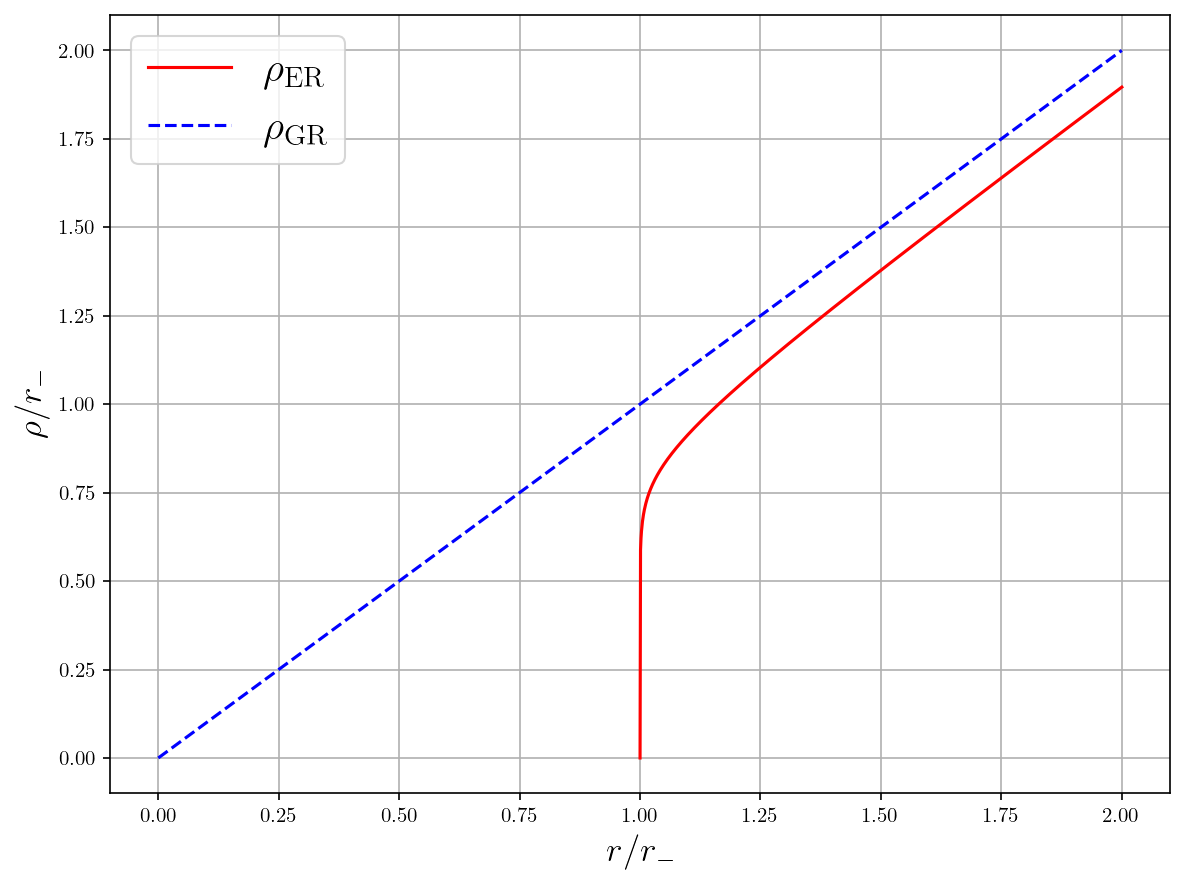
\includegraphics[width=\linewidth]{images/rho.png}
        \caption{}
        \label{subfig:rho}
    \end{subfigure}
    \caption{Behavior of the areal radius $\rho$ in GR and ER. (\ref{subfig:horizons}) Horizons in $r$ and $\rho$ coordinates as a function of $Q/M$ for GR and ER. $\rho_\mrm{GR}$ is not shown as it coincides with $r_\mrm{GR}$. (\ref{subfig:rho}) The $\rho$ coordinate as a function of the $r$ coordinate.}
    \label{fig:areal}
\end{figure}


%%%%%%%%%%%%%%%%%%%%%%%%%%%%%%%%%%%%%%%%%%%%%%%%%%%%%%%%%%%%%%%%%%%%%%%%



\section{Photon Orbit Analysis}

First, we want to look at the simplest cases: photons. It is easier because photons follow null geodesics of the metric both in GR and in ER.

\subsection{Trajectories Comparison}

The first thing we can do is to plot the trajectories of photons around black holes of different charges and for both theories. In figure (\ref{fig:null_geod}) we show the difference between using the $r$ coordinate and the $\rho$ coordinate defined above. We choose the initial condition $r_0/M = 3$ and $\rho_0/M = 3$ which corresponds to the photon sphere in GR. The initial conditions are matched in terms of the chosen tangent components $k_t$, $k_r$ (or $k_\rho$) and $k_\varphi$; therefore, these plots should be interpreted as qualitative trajectory comparisons rather than as fixed-impact-parameter lensing observables. We can see the two theories agree much more when we use the areal radius $\rho$. When we use the $r$ coordinate, the trajectories diverge much faster.

\begin{figure}[h]
    \centering
    \begin{subfigure}{0.48\linewidth}
        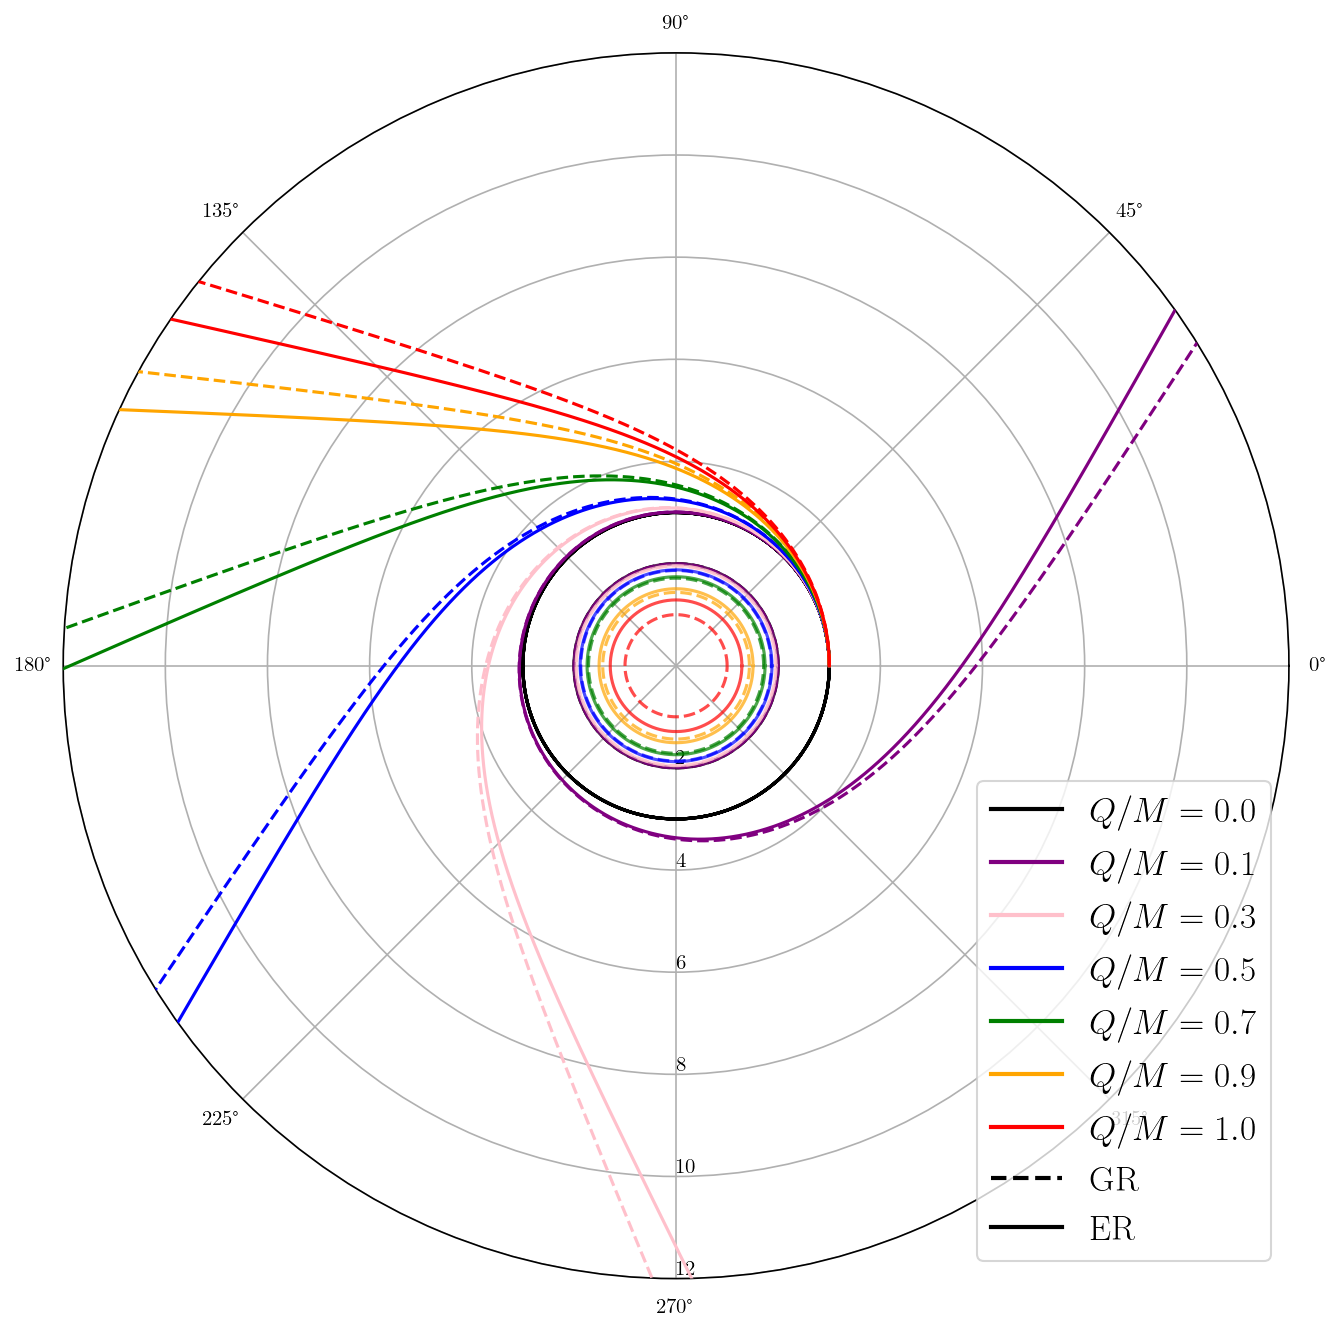
\includegraphics[width=\linewidth]{images/NullGeodesics_rCoordinate.png}
        \caption{}
        \label{subfig:null_r}
    \end{subfigure}
    \begin{subfigure}{0.48\linewidth}
        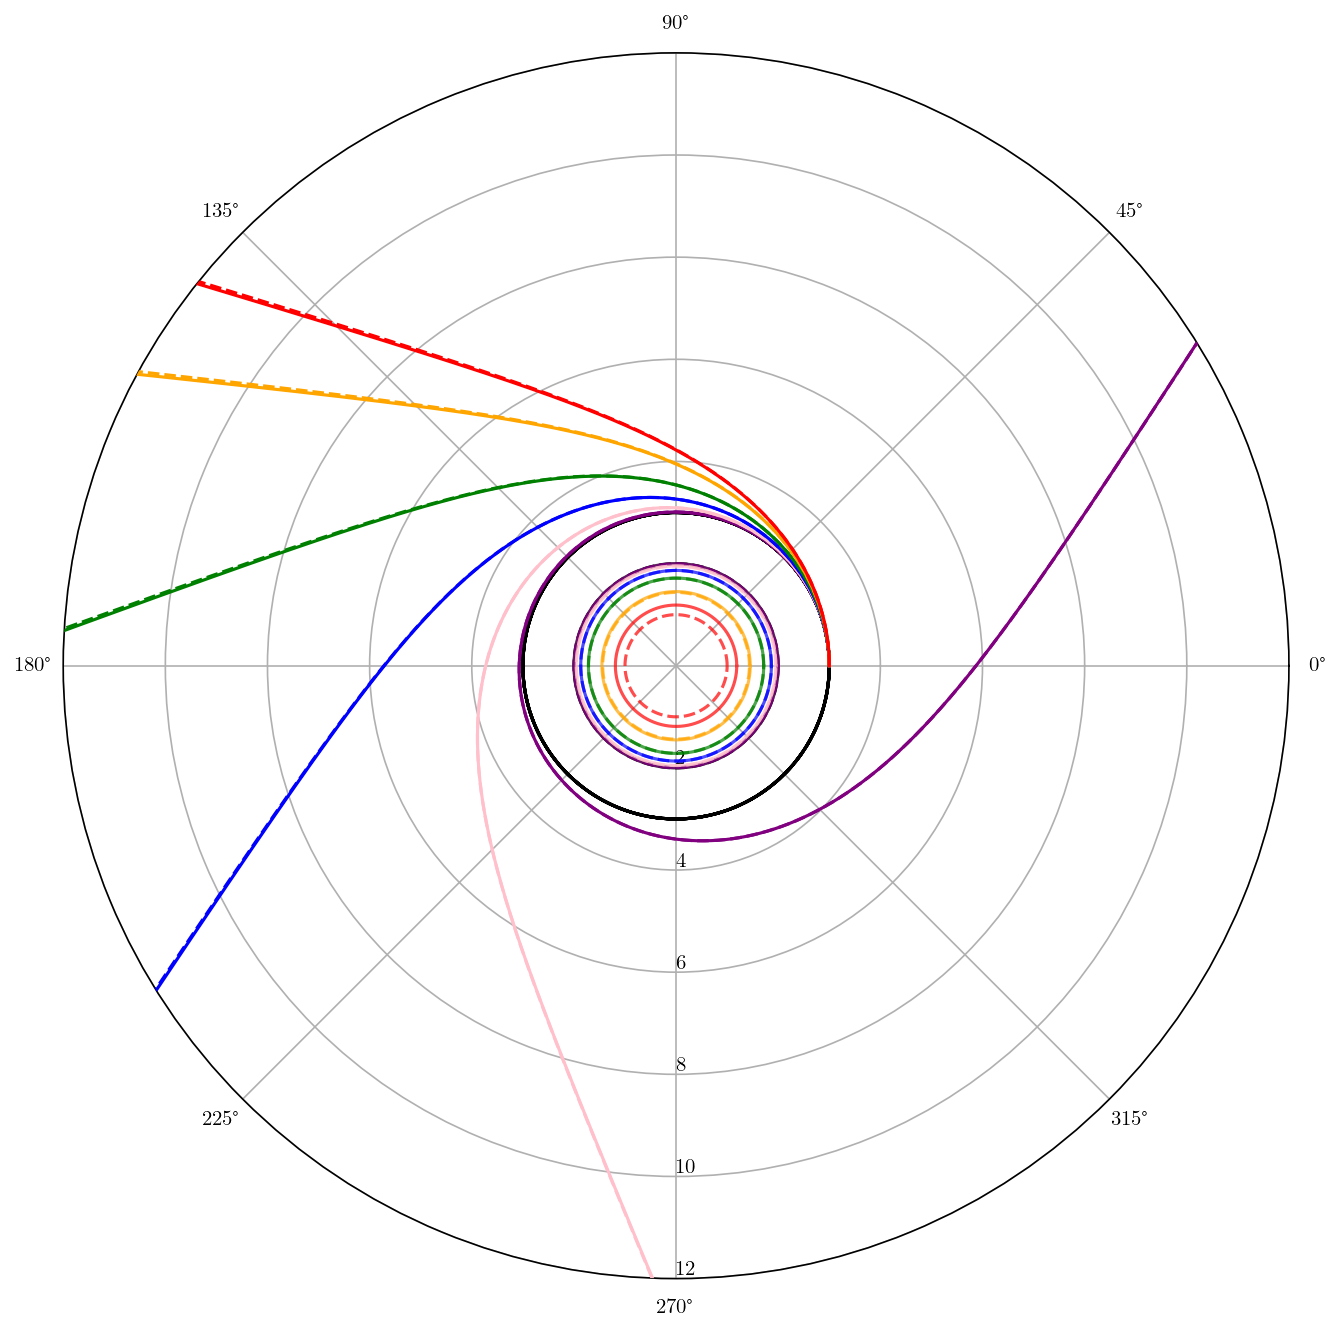
\includegraphics[width=\linewidth]{images/NullGeodesics_rhoCoordinate.png}
        \caption{}
        \label{subfig:null_rho}
    \end{subfigure}
    \caption{Null geodesics around charged black holes in GR and ER. (\ref{subfig:null_r}) We use the coordinate $r$. (\ref{subfig:null_rho}) We use the coordinate $\rho$.}
    \label{fig:null_geod}
\end{figure}
However, this analysis can be biased by the size of the black hole. Indeed, for a given mass and charge, GR and ER predict different horizons given by equations (\ref{HorizonsRN}) and (\ref{HorizonsER}) respectively. Therefore normalizing distances by the horizon radius $\rho_+$ seems more relevant. The result is shown in figure (\ref{fig:null_horizon}) where the distances are rescaled such that every black hole has a horizon radius equal to 1. We specifically choose an initial condition for which photons can either fall into the black hole or escape to infinity depending on the charge-to-mass ratio of the black hole. For example, when the charge vanishes, we have a Schwarzschild black hole and the result is expected since we start above the photon sphere which lies at $\rho = 1.5\rho_+$. However, for $Q/M = 1$, which corresponds to a GR extremal black hole but not an ER extremal black hole, the photon falls in the black hole. This can play a role in the study of gravitational lensing which we will discuss later.

\begin{figure}
    \centering
    
\includegraphics[width=0.5\linewidth]{images/NullGeodesics_Horizon.png}
    \caption{Null geodesics with normalization with respect to horizon radius. The initial condition is $\rho_0/\rho_+ = 1.6$.}
    \label{fig:null_horizon}
\end{figure}
We can check the validity of our numerical analysis by looking at the numerical value of the normalization of the $k$ vector defined by $k^\mu = \frac{\mrm dx^\mu}{\mrm d\lambda}$ where $\lambda$ is an affine parameter. In figure (\ref{fig:error}), we show the absolute value of the pseudo-norm of the $k$ vector with respect to the distance to the horizon. The results are fully compatible with $k_\mu k^\mu = 0$ along all the trajectory. The error increases as the photon travels closer to the horizon. This is logical since the spacetime is more curved near the horizon. However, it is worth pointing out that the error is larger for GR than for ER. It is quite unexpected knowing that ER is mathematically more complex than GR and more non-linear. Away from the black hole, the error remains lower than $10^{-9}$ which is numerically acceptable.

\begin{figure}[h]
    \centering
    
\includegraphics[width=0.8\linewidth]{images/Error_Horizon.png}
    \caption{Normalization error with respect to the distance to the horizon for $Q/M = 1$.}
    \label{fig:error}
\end{figure}

\subsection{Effective Potential and Photon Sphere}

Now, we want to have a look at the effective potential the way it is defined in \cite{Gourgoulhon2026BlackHoles}. The expression of the effective potential for photons is given in appendix \ref{appendix:effpot}. For GR, it is:

\begin{equation}
    V_\mrm{eff}^\mrm{GR}(r) = \frac{1}{r^2}\paren{1 - \frac{r_+}{r}}\paren{1 - \frac{r_-}{r}},
\end{equation}
and for ER:

\begin{equation}
    V_\mrm{eff}^\mrm{ER}(r) = \frac{1}{r^2}\paren{1 - \frac{r_+}{r}}\paren{1 - \frac{r_-}{r}}^{9/13}.
\end{equation}
In figure \ref{fig:eff_pot}, we show the effective potentials in $r$ coordinate and in $\rho$ coordinate. In the same way, we can see GR and ER agree more when we use the areal radius. This allows us to study the photon sphere in both theories. The photon sphere is defined as the radius $\rho_\mrm{ph}$ such that $\frac{\mrm dV_\mrm{eff}}{\mrm dr}(r(\rho_\mrm{ph})) = 0$ and $\frac{\mrm d^2V_\mrm{eff}}{\mrm dr^2}(r(\rho_\mrm{ph})) < 0$. We can actually obtain analytic expressions for $r_\mrm{ph} = r(\rho_\mrm{ph})$. For GR, it is given by:

\begin{equation}
    r_\mrm{ph}^\mrm{GR} = \frac{1}{2}\paren{3M + \sqrt{9M^2 - 8Q^2}},
\end{equation}
which recovers $r_\mrm{ph} = 3M = \frac{3}{2}r_+$ for an uncharged black hole. For ER, we can show the following expression:

\begin{equation}
    r_\mrm{ph}^\mrm{ER} = \frac{1}{4}\paren{\frac{35}{13}r_- + 3r_+ + \sqrt{\paren{\frac{35}{13}r_- + 3r_+}^2 - \frac{384}{13}r_-r_+}},
\end{equation}
which also gives $r_\mrm{ph} = \frac{3}{2}r_+$ in the neutral case.

\begin{figure}[h]
    \centering
    \begin{subfigure}{0.48\linewidth}
        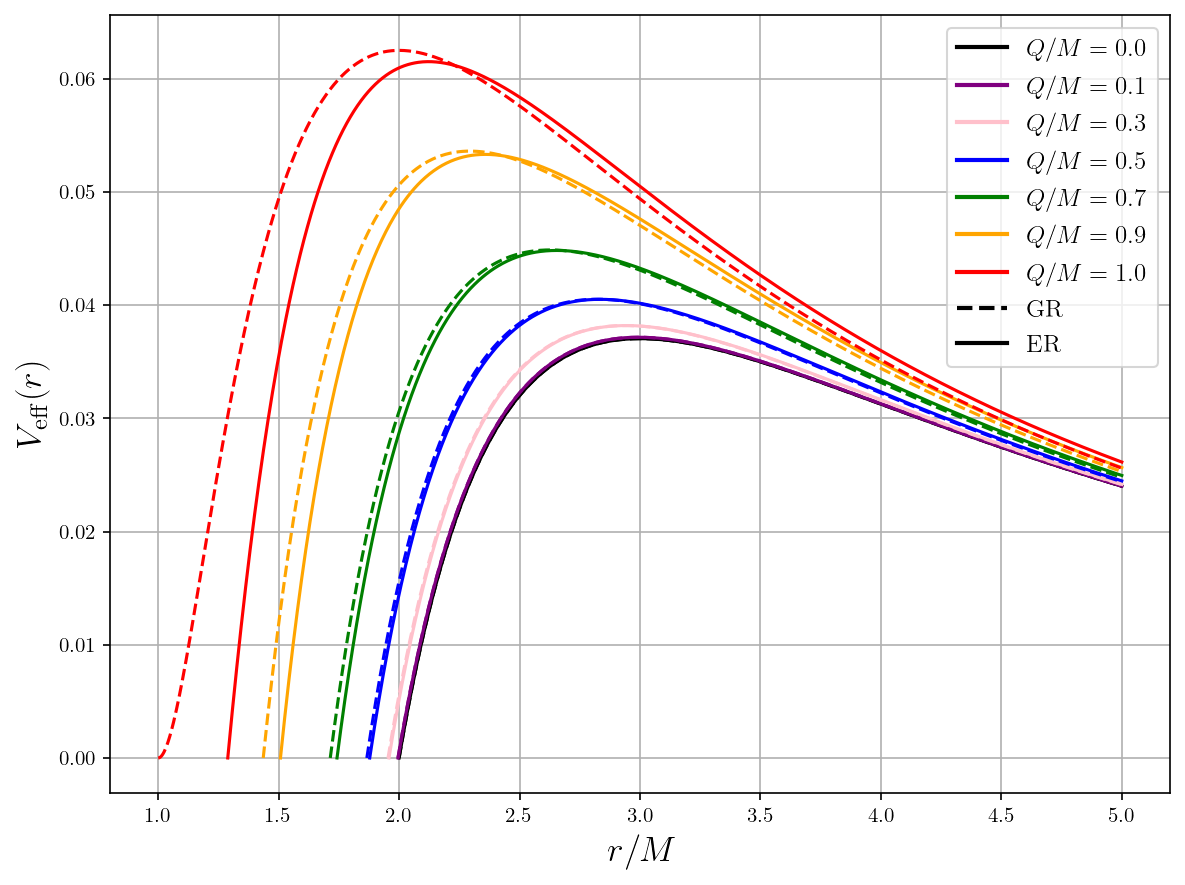
\includegraphics[width=\linewidth]{images/EffectivePotentials_rCoordinate.png}
        \caption{}
        \label{subfig:eff_r}
    \end{subfigure}
    \begin{subfigure}{0.48\linewidth}
        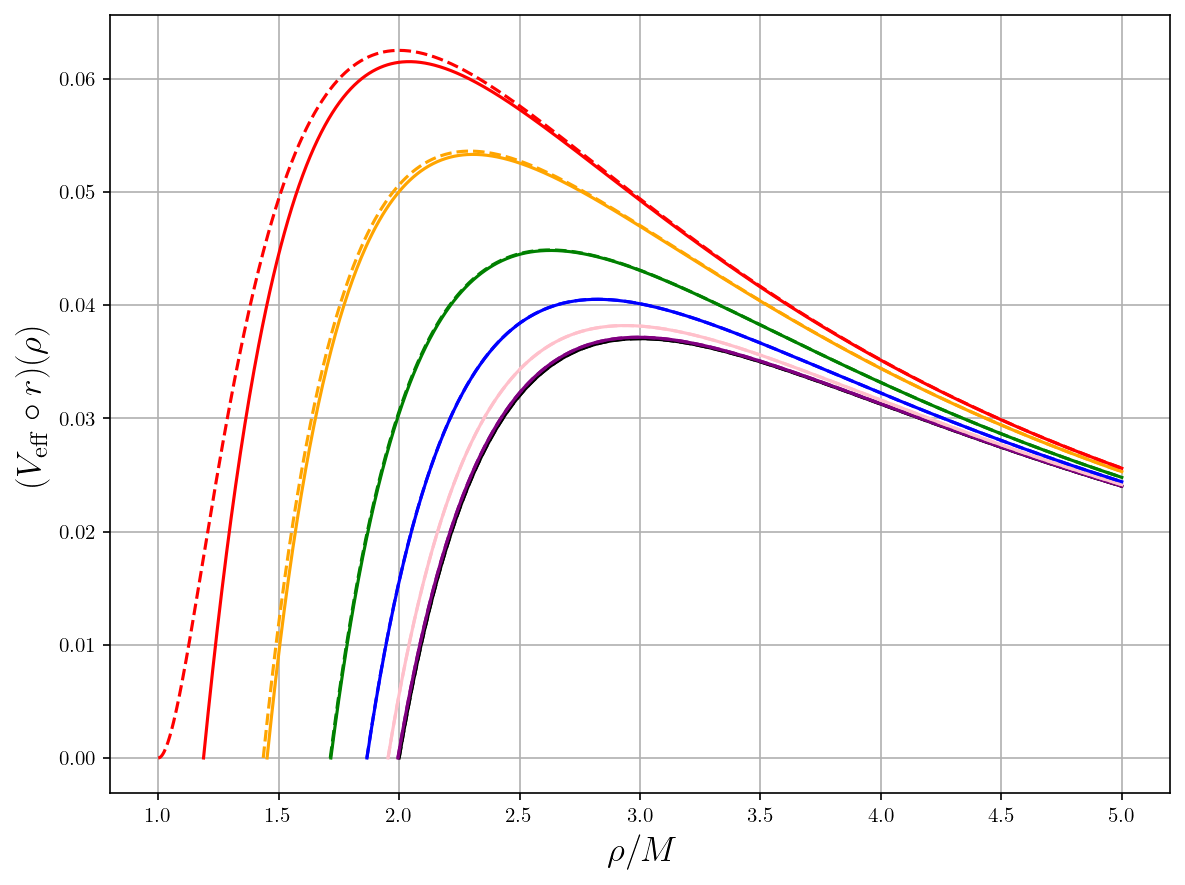
\includegraphics[width=\linewidth]{images/EffectivePotentials_Mass.png}
        \caption{}
        \label{subfig:eff_rho}
    \end{subfigure}
    \caption{Effective potentials in $r$ coordinate (\ref{subfig:eff_r}) and in $\rho$ coordinate (\ref{subfig:eff_rho}) normalized with the mass of the black hole.}
    \label{fig:eff_pot}
\end{figure}
In figure \ref{fig:photon_sphere}, we show the photon sphere compared to the horizon with respect to the charge-to-mass ratio. We can only see a difference between the two theories for highly charged black holes. For a GR extremal black hole (i.e. $Q=M$), ER predicts a smaller photon sphere compared to the horizon radius. For an ER extremal black hole (i.e. $Q/M=\sqrt{143/132}$), we have $\rho_\mrm{ph}/M = 2\paren{\frac{11}{24}}^{1/13} \approx 1.88$.


\begin{figure}
    \centering
    \begin{subfigure}{0.48\linewidth}
        
\includegraphics[width=\linewidth]{images/PhotonSphere_Mass.png}
        \caption{}
        \label{subfig:photon_mass}
    \end{subfigure}
    \begin{subfigure}{0.48\linewidth}
        
\includegraphics[width=\linewidth]{images/PhotonSphere_Horizon.png}
        \caption{}
        \label{subfig:photon_horizon}
    \end{subfigure}
    \caption{Photon sphere radius with respect to the charge-to-mass ratio. (\ref{subfig:photon_mass}) The radius is normalized with the mass of the black hole and we also show the horizon. (\ref{subfig:photon_horizon}) The radius is normalized with the horizon.}
    \label{fig:photon_sphere}
\end{figure}

\subsection{Deflection Angle and Lensing}

In this section, we discuss lensing in both theories. In particular, we can compute the deflection angle $\hat\alpha$ that is defined by \cite{Bozza_2002}:

\begin{equation}
    \hat\alpha(b) = 2\int_{r_0}^\infty \frac{b \mrm dr}{\rho^2(r)\sqrt{1 - b^2V_\mrm{eff}(r)}} - \pi,
\end{equation}
where $b$ is the impact parameter and $r_0$, defined by $V_\mrm{eff}(r_0) = b^{-2}$, is the outer radial turning point. This expression applies for scattering trajectories with $b > b_\mrm{crit}$ with $b_\mrm{crit}$ the critical impact parameter defined by:

\begin{equation}
    b_\mrm{crit} = \frac{1}{\sqrt{V_\mrm{eff}(r_\mrm{ph})}}.
\end{equation}
The results are shown in figure \ref{fig:lensing} where we plot $\hat\alpha$ and $b_\mrm{crit}$. No appreciable difference is visible for low charge black holes. However, for a GR extremal black hole, ER predicts a higher critical impact parameter.


\begin{figure}[h]
    \centering
    \begin{subfigure}{0.48\linewidth}
        
\includegraphics[width=\linewidth]{images/DeflectionAngle_vs_ImpactParameter_Mass.png}
        \caption{}
        \label{subfig:angle}
    \end{subfigure}
    \begin{subfigure}{0.48\linewidth}
        
\includegraphics[width=\linewidth]{images/CriticalImpactParameter_vs_Charge.png}
        \caption{}
        \label{subfig:bcrit}
    \end{subfigure}
    \caption{(\ref{subfig:angle}) Deflection angle $\hat\alpha$ with respect to the impact parameter $b/M$. (\ref{subfig:bcrit}) Critical impact parameter as a function of $Q/M$ for GR and ER.}
    \label{fig:lensing}
\end{figure}



%%%%%%%%%%%%%%%%%%%%%%%%%%%%%%%%%%%%%%%%%%%%%%%%%%%%%%%%%%%%%%%%%%%


\section{Dynamics of Massive Particles}

Now that we studied the dynamics of massless particles (photons), we want to analyze the dynamics of massive particles. The key difference between the two is that massive particles do not follow geodesics of the metric in entangled frame. We therefore work in the Einstein frame where the complete dynamics is encoded in the metric without any additional scalar field. The equations of motion in entangled frame are derived in appendix \ref{appendix:conformal}.

\subsection{Trajectories}

We next examine trajectories of massive particles around a charged black hole. In figure \ref{fig:massive}, we show some trajectories with initial conditions chosen such that the neutral case is located at the ISCO radius, that we will discuss just after. Again, we can see a slight difference between GR and ER only when the charge is close to the mass (in proper units). The right plot shows that when particles start from the same point compared to the size of the black hole, they fall into the black hole after fewer revolutions as the charge increases.

\begin{figure}[h]
    \centering
    \begin{subfigure}{0.48\linewidth}
        
\includegraphics[width=\linewidth]{images/Massive_Mass.png}
        \caption{}
        \label{subfig:massive_mass}
    \end{subfigure}
    \begin{subfigure}{0.48\linewidth}
        
\includegraphics[width=\linewidth]{images/Massive_Horizon.png}
        \caption{}
        \label{subfig:massive_horizon}
    \end{subfigure}
    \caption{Trajectories of massive test particles around charged black holes in GR and ER. (\ref{subfig:massive_mass}) We normalize distances with the mass of the black hole. (\ref{subfig:massive_horizon}) We normalize distances with the horizon radius.}
    \label{fig:massive}
\end{figure}

\subsection{ISCO Radius}

The ISCO radius $r_\mrm{ISCO}$ is the smallest marginally stable circular orbit. It means it verifies the relations $V_\mrm{eff}'(r_\mrm{ISCO}) = V_\mrm{eff}''(r_\mrm{ISCO}) = 0$. It is the solution of the equation:

\begin{equation}
    Mr^3 - 6M^2r^2 + 9MQ^2r - 4Q^4 = 0,
\end{equation}
for GR and:

\begin{align}
    &(2197r_+ + 1859 r_-)r^4 \notag \\
    &- (6591 r_+^2 + 13351r_+r_- + 6578r_-^2)r^3 \notag \\
    &+ (24336r_+^2r_- + 25740r_+r_-^2 + 4620 r_-^3)r^2 \notag \\
    &- (31668r_+^2r_-^2 + 14388r_+r_-^3)r \notag \\
    &+ 13824r_+^2r_-^3=0,
\end{align}
for ER. The derivation of these is given in appendix \ref{appendix:ISCO}. We can numerically solve them and study their solutions for different charges. The figure \ref{fig:ISCO} shows the ISCO radius as $Q/M$ increases and the difference between both theories. This difference will play a role in our phenomenology study.

\begin{figure}[h]
    \centering
    \begin{subfigure}{0.48\linewidth}
        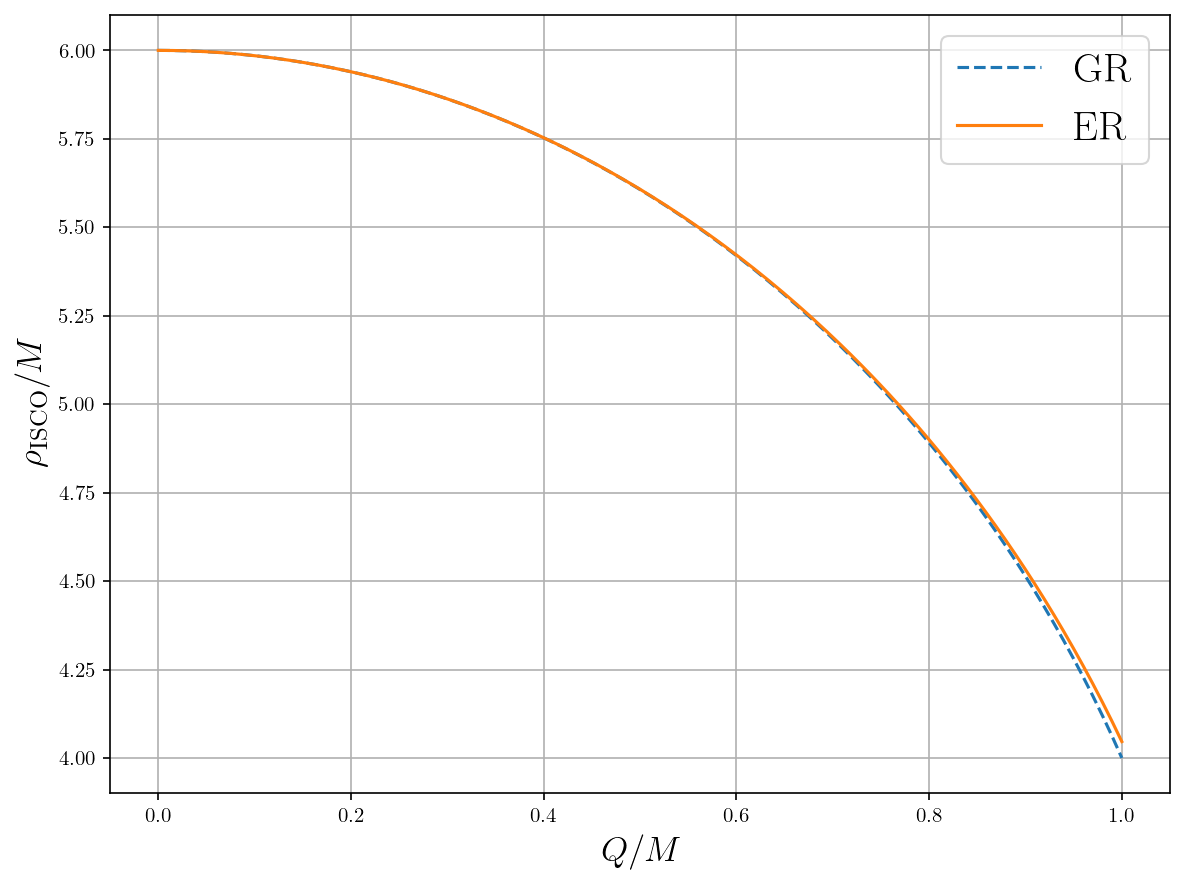
\includegraphics[width=\linewidth]{images/ISCO.png}
        \caption{}
        \label{subfig:ISCO}
    \end{subfigure}
    \begin{subfigure}{0.48\linewidth}
        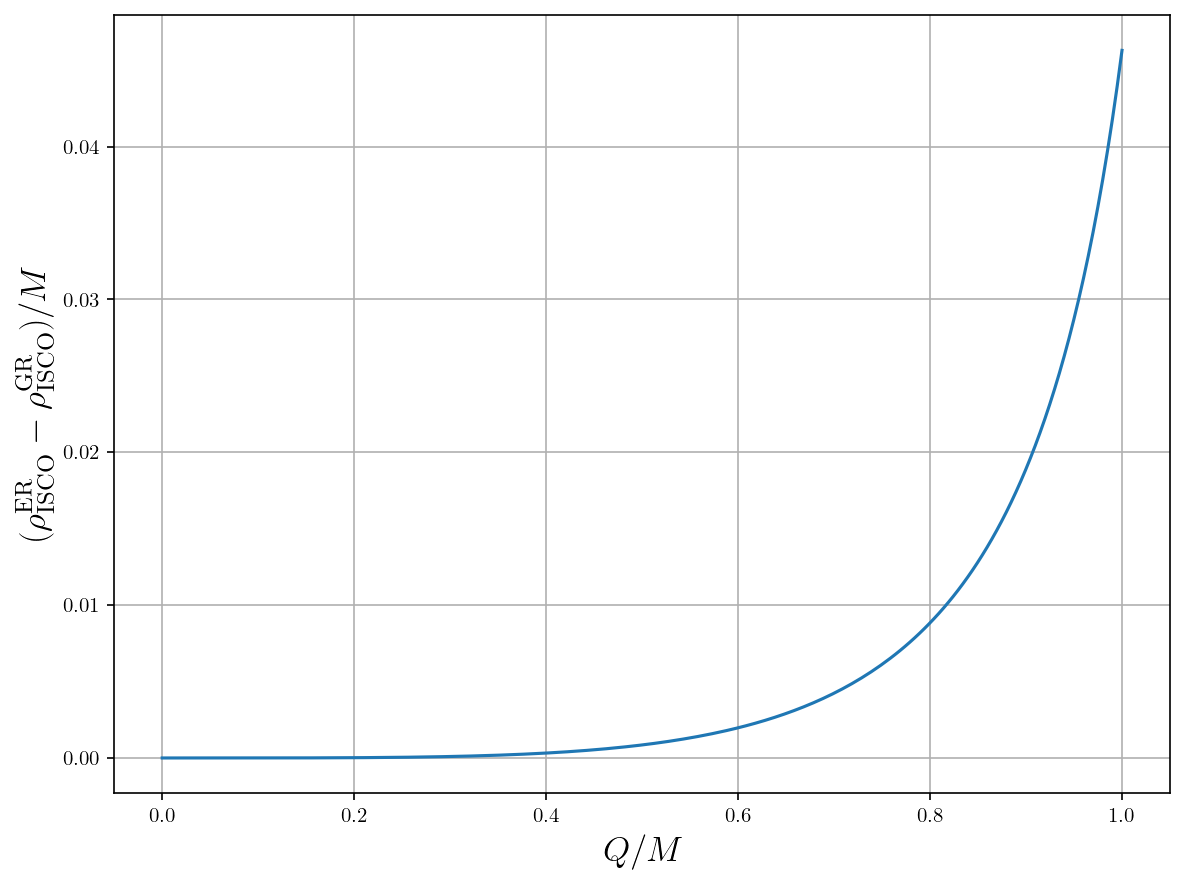
\includegraphics[width=\linewidth]{images/ISCO2.png}
        \caption{}
        \label{subfig:ISCO2}
    \end{subfigure}
    \caption{ISCO radius analysis. (\ref{subfig:ISCO}) ISCO Radius with respect to the charge-to-mass ratio for both theories. (\ref{subfig:ISCO2}) Difference between the two.}
    \label{fig:ISCO}
\end{figure}


\subsection{Kepler's Third Law}

Before diving into black hole phenomenology, we want to write a Kepler's third law equivalent for charged black holes in GR and in ER. In classical mechanics, the Kepler's third law is the relation between the radius of a circular orbit $r$ and the angular velocity $\Omega$ of the particle following this orbit, usually written as $T^2/r^3 = 4\pi^2/M$ with $T$ the period of revolution. In GR, the equivalent of this relation for a charged black hole is given by:

\begin{equation}
    \Omega_\mrm{GR}^2 = \frac{M}{r^3}-\frac{Q^2}{r^4},
\end{equation}
which recovers the classical relation $\Omega^2r^3 = M$ with a contribution proportional to $1/r^4$ due to the charge of the black hole. In ER, the Kepler's third law reads:

\begin{equation}
    \Omega_\mrm{ER}^2 = \frac{\paren{1 - \frac{r_-}{r}}^{9/13}}{1 - \frac{12}{13}\frac{r_-}{r}}\Omega_\mrm{GR}^2,
\end{equation}
which is equal to $\Omega_\mrm{GR}^2$ when the charge is zero. The derivation of these relations is given in appendix \ref{appendix:kepler}. The figure \ref{fig:kepler} shows the angular velocity as a function of the radius for different charge-to-mass ratios. For the GR extremal case, we can see that the angular velocity collapses as the radius decreases. This turnover appears when the charge term wins over the mass term. However this turnover appears below the photon sphere and therefore is not observable.

\begin{figure}
    \centering
    \begin{subfigure}{0.48\linewidth}
        
\includegraphics[width=\linewidth]{images/Kepler.png}
        \caption{}
        \label{subfig:Kepler}
    \end{subfigure}
    \begin{subfigure}{0.48\linewidth}
        
\includegraphics[width=\linewidth]{images/Kepler2.png}
        \caption{}
        \label{subfig:Kepler2}
    \end{subfigure}
    \caption{Angular velocity of a massive test particle following a circular orbit with respect to the areal radius.}
    \label{fig:kepler}
\end{figure}








%%%%%%%%%%%%%%%%%%%%%%%%%%%%%%%%%%%%%%%%%%%%%%%%%%%%%%%%%%%%%%%%%%

\section{Black Hole Phenomenology}

In this section, we try answering the following questions: For some given observational data, what are the properties of the black hole predicted by both theories? And how wrong are we when we use a model based on GR if the data was generated by ER?

\subsection{Circular Orbit}

We first consider an idealized situation in which several neutral test bodies follow circular orbits around the same black hole. We assume that the areal radii $\rho_i$ and angular velocities $\Omega_i$ of these bodies have been inferred from their observed trajectories. In practice, these quantities would be obtained from an astrometric and spectroscopic fit, rather than measured directly. In the present analysis, the radii are assumed to be known exactly and an uncertainty is assigned only to the angular velocities.

The purpose of this analysis is to address the two questions introduced above. First, can the mass $M$ and charge-to-mass ratio
\begin{equation}
q \equiv \frac{|Q|}{M},
\end{equation}
be recovered from a collection of circular orbits? Second, if the data are generated according to ER but interpreted using the GR Kepler law, how strongly are the inferred values of $M$ and $q$ biased?

\subsubsection{Generation and fitting of mock data}

The mock observations are generated using the ER Kepler law derived previously. For a chosen pair $(M_{\mrm{true}},q_{\mrm{true}})$, we randomly draw $N=8$ areal radii in the interval
\begin{equation}
1.01\max\left(\rho_{\mrm{ISCO}}^{\mrm{GR}}, \rho_{\mrm{ISCO}}^{\mrm{ER}}\right) <\rho_i<15M_{\mrm{true}},
\end{equation}
which covers a variation of 5.04\% in the scalar field ($\phi\in \bracket{1.0179, 1.0719}$). The lower limit ensures that all generated bodies are located outside the ISCO predicted by both theories and can therefore follow stable circular orbits.

At each radius, the exact angular velocity is computed from
\begin{equation}
\Omega_{i,\mrm{true}} = \Omega_{\mrm{ER}} \left(\rho_i; M_{\mrm{true}}, q_{\mrm{true}} \right).
\end{equation}
Gaussian noise is then added according to
\begin{equation}
\Omega_{i,\mrm{obs}} = \Omega_{i,\mrm{true}} + \epsilon_i, \ \ \ \epsilon_i \sim \mcal N\left(0,\sigma_{\Omega_i}^2\right),
\end{equation}
where a relative uncertainty of one percent is assumed:
\begin{equation}
\sigma_{\Omega_i} = 0.01\Omega_{i,\mrm{true}}.
\end{equation}
The same mock data are fitted independently with the ER and GR expressions of the Kepler law. For a theory $X\in(\mrm{ER},\mrm{GR})$, the fitted parameters are obtained by minimizing
\begin{equation}\label{chi2Circular}
\chi_X^2(M,q) = \sum_{i=1}^{N}\frac{\left[\Omega_{i,\mrm{obs}} - \Omega_X(\rho_i;M,q) \right]^2}{\sigma_{\Omega_i}^2}.
\end{equation}
We can estimate the uncertainties on $M$ and $q$. Figure \ref{fig:mock_circular} shows one realization generated with
\begin{equation}
M_{\mrm{true,ER}}=1,\ \ \ q_{\mrm{true,ER}}=0.9.
\end{equation}
The two fitted curves are almost indistinguishable on the scale of the figure. The ER fit gives
\begin{equation}
M_{\mrm{ER}} = 0.9799\pm0.0183,\ \ \ q_{\mrm{ER}} = 0.8712\pm0.0537,
\end{equation}
as a 68.27\% confidence interval, whereas the GR fit gives
\begin{equation}
M_{\mrm{GR}} = 0.9795\pm0.0182,\ \ \ q_{\mrm{GR}} = 0.8679\pm0.0529.
\end{equation}
Both models therefore recover values compatible with the true parameters except for the mass that is slightly underestimated. For this particular realization, the minimum chi-squared values are
\begin{equation}
\chi_{\mrm{ER}}^2=5.399,\ \ \ \chi_{\mrm{GR}}^2=5.393.
\end{equation}
Since two parameters are fitted to eight measurements, the number of degrees of freedom is $\nu=6$. The values obtained for this individual realization are quite compatible with this prediction. The very small difference between the two values does not provide any preference for one theory.

\begin{figure}[h]
\centering

\includegraphics[width=0.72\linewidth]{images/MockData.png}
\caption{One realization of ER-generated circular-orbit data for $M_{\mrm{true}}=1$ and $q_{\mrm{true}}=0.9$. The vertical error bars correspond to a relative uncertainty $\sigma_\Omega/\Omega=1\%$. The solid line is the best ER fit and the dashed line is the best GR fit. The two curves almost completely overlap.}
\label{fig:mock_circular}
\end{figure}

\subsubsection{Statistical distributions}

The procedure is then repeated for 1000 independent realizations. In each realization, both a new set of radii and a new set of Gaussian perturbations are generated. Figure \ref{fig:circular_distributions} shows the resulting distributions of the fitted mass and charge-to-mass ratio for $q_{\mrm{true}}=0.9$.

For the ER model, the ensemble averages and standard deviations are
\begin{equation}
\left\langle M_{\mrm{fit}}\right\rangle_{\mrm{ER}} = 0.9998,\ \ \ \sigma(M_{\mrm{fit}})_{\mrm{ER}} = 0.0236,\ \ \ \left\langle q_{\mrm{fit}}\right\rangle_{\mrm{ER}} = 0.8846,\ \ \ \sigma(q_{\mrm{fit}})_{\mrm{ER}} = 0.1161.
\end{equation}
For the GR model, one obtains
\begin{equation}
\left\langle M_{\mrm{fit}}\right\rangle_{\mrm{GR}} = 0.9987,\ \ \ \sigma(M_{\mrm{fit}})_{\mrm{GR}} = 0.0224,\ \ \ \left\langle q_{\mrm{fit}}\right\rangle_{\mrm{GR}} = 0.8788,\ \ \ \sigma(q_{\mrm{fit}})_{\mrm{GR}} = 0.1122.
\end{equation}
The mass is recovered with a typical statistical dispersion of approximately $2.3\%$, whereas the charge-to-mass ratio is less precisely determined. The distributions obtained with GR and ER strongly overlap. Consequently, with the adopted radial interval and one-percent uncertainty on $\Omega$, the statistical fluctuations are substantially larger than the difference between the two theoretical predictions. The average minimum chi-squared values are
\begin{equation}
\left\langle\chi_{\mrm{ER}}^2\right\rangle
=6.224,\ \ \ \left\langle\chi_{\mrm{GR}}^2\right\rangle
=6.250,
\end{equation}
in agreement with the expected value $\nu=6$. Therefore, although the observations are generated with ER, the GR model provides a statistically acceptable fit.

\begin{figure}[h]
\centering
\begin{subfigure}{0.48\linewidth}

\includegraphics[width=\linewidth]{images/MassDistrib.png}
\caption{}
\label{subfig:circular_mass_distribution}
\end{subfigure}
\begin{subfigure}{0.48\linewidth}

\includegraphics[width=\linewidth]{images/ChargeDistrib.png}
\caption{}
\label{subfig:circular_charge_distribution}
\end{subfigure}
\caption{Distributions of the fitted parameters over 1000 independent ER-generated realizations with $M_{\mrm{true}}=1$ and $q_{\mrm{true}}=0.9$. The dashed vertical lines indicate the true values. (\ref{subfig:circular_mass_distribution}) Distribution of the fitted mass. (\ref{subfig:circular_charge_distribution}) Distribution of the fitted charge-to-mass ratio. The ER and GR distributions strongly overlap.}
\label{fig:circular_distributions}
\end{figure}

At low charge, the two theories are even more difficult to distinguish. The charge contribution to the angular velocity is subdominant at the considered radii, and the fitted value of $q$ becomes poorly constrained. For example, for $q_{\mrm{true}}=0.3$, the standard deviation of the fitted charge-to-mass ratio is approximately $0.27$. The constraint improves as the charge increases, reaching a standard deviation of approximately $0.07$ for $q_{\mrm{true}}=1$. This does not mean that low charges produce a large physical bias; rather, the orbital frequencies are not sufficiently sensitive to $q$ to measure it accurately in this regime.

\subsubsection{Low noise discrimination test}

The distributions shown above contain both the difference between the theories and the random observational noise. To isolate the systematic error caused only by the use of the wrong model, we also fit ER data with the GR expression for a very low uncertainty $\sigma_\Omega / \Omega = 10^{-5}$. For this calculation, the exact ER angular velocity is evaluated for 1000 realizations of 100 radii between roughly the largest ISCO and $15M$. The corresponding distributions are given in figure \ref{fig:distrib_noiseless} where we see that true values of $M$ and $q$ are recovered much better than before.

\begin{figure}[h]
    \centering
    \begin{subfigure}{0.48\linewidth}
        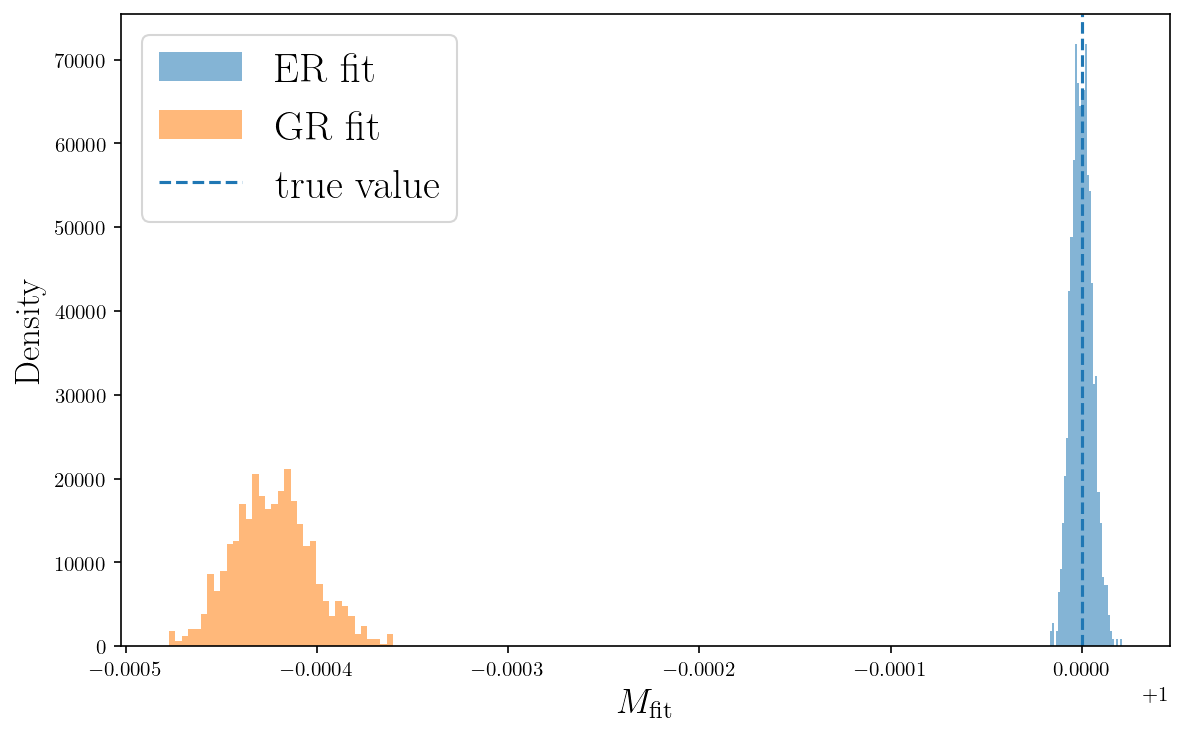
\includegraphics[width=\linewidth]{images/MassDistrib_Noiseless.png}
        \caption{}
        \label{subfig:massdistrib_noiseless}
    \end{subfigure}
    \begin{subfigure}{0.48\linewidth}
        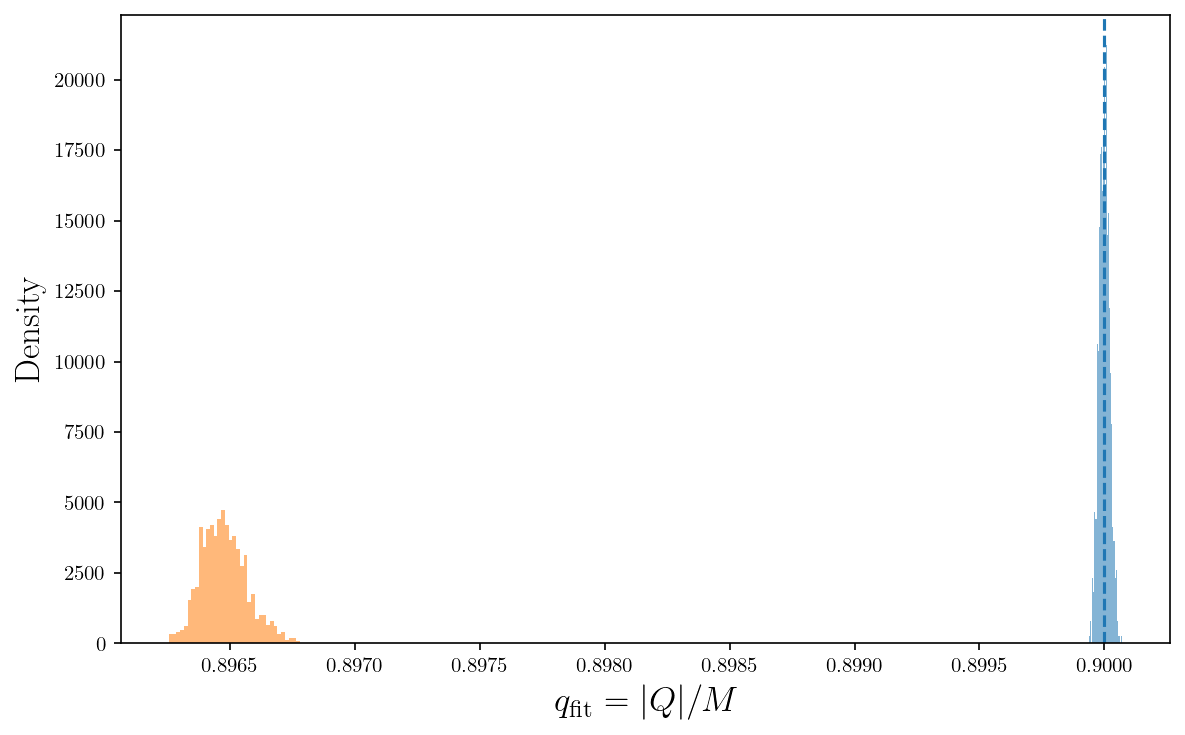
\includegraphics[width=\linewidth]{images/ChargeDistrib_Noiseless.png}
        \caption{}
        \label{subfig:chargedistrib_noiseless}
    \end{subfigure}
    \caption{Distributions of the fitted parameters over 1000 independent low noise ER-generated realizations with $M_{\mrm{true}}=1$ and $q_{\mrm{true}}=0.9$. The dashed vertical lines indicate the true values. (\ref{subfig:massdistrib_noiseless}) Distribution of the fitted mass. (\ref{subfig:chargedistrib_noiseless}) Distribution of the fitted charge-to-mass ratio.}
    \label{fig:distrib_noiseless}
\end{figure}
One obtains

\begin{equation}
\left\langle M_{\mrm{fit}}\right\rangle_{\mrm{ER}} = 1.000,\ \ \ \sigma(M_{\mrm{fit}})_{\mrm{ER}} = 6\times 10^{-6},\ \ \ \left\langle q_{\mrm{fit}}\right\rangle_{\mrm{ER}} = 0.9000,\ \ \ \sigma(q_{\mrm{fit}})_{\mrm{ER}} = 2\times 10^{-5},
\end{equation}
and

\begin{equation}
\left\langle M_{\mrm{fit}}\right\rangle_{\mrm{GR}} = 0.9996,\ \ \ \sigma(M_{\mrm{fit}})_{\mrm{GR}} = 2.1\times 10^{-5},\ \ \ \left\langle q_{\mrm{fit}}\right\rangle_{\mrm{GR}} = 0.8965,\ \ \ \sigma(q_{\mrm{fit}})_{\mrm{GR}} = 9.1\times 10^{-5}.
\end{equation}
In this case, the standard deviations are much higher for GR than for ER. Moreover, GR does not recover the true value under the given uncertainties. At this level of precision, the GR fit leads to a statistically significant bias in the inferred parameters. To quantify how much GR and ER can be discriminated from each other, we consider 

\begin{equation}
    \langle\Delta\chi^2\rangle = \langle\chi^2_\mrm{GR,min}\rangle - \langle\chi^2_\mrm{ER,min}\rangle = 739.596 - 98.130 = 641.466,
\end{equation}
which strongly disfavors the GR fit in this low-noise setup. Although both $\sigma_\Omega / \Omega$ and $N$ are changed here, an additional test shows that the difference is essentially driven by the decrease in $\sigma_\Omega/\Omega$. This is done for a high charge-to-mass ratio. We want to see the results for different charges. The results are given in figure \ref{fig:bias} where we show the corresponding uncertainties. We can see GR always underestimates the parameters but still recovers the true values for low charges. This is logical since ER approaches GR in the neutral limit.

\begin{figure}[h]
    \centering
    \begin{subfigure}{0.48\linewidth}
        
\includegraphics[width=\linewidth]{images/MassBias.png}
        \caption{}
        \label{subfig:massbias}
    \end{subfigure}
    \begin{subfigure}{0.48\linewidth}
        
\includegraphics[width=\linewidth]{images/ChargeBias.png}
        \caption{}
        \label{subfig:chargebias}
    \end{subfigure}
    \caption{Parameter bias obtained in the low-noise circular-orbit test. The ER-generated data are fitted with both the ER and GR models. The GR fit systematically underestimates both $M$ and $q$, with a bias increasing with $q_\mrm{true}$. (\ref{subfig:massbias}) Relative bias on the inferred mass. (\ref{subfig:chargebias}) Bias on the inferred charge-to-mass ratio.}
    \label{fig:bias}
\end{figure}



\subsection{General Orbit}

The circular-orbit analysis considered above uses only the relation between one characteristic radius and one angular velocity. General bound orbits may in principle provide more information than circular ones. While a circular orbit probes the relation between the angular velocity and the metric at one fixed radius, an eccentric orbit explores a continuous interval between its periastron and apoastron. It may therefore provide several observables, including the radial period, the variation of the orbital velocity and the relativistic advance of the periastron. In particular, the repeated accumulation of a difference in periastron precession could make small deviations between GR and ER observable over many revolutions.

A preliminary numerical study was performed by generating ER orbits and comparing their radial periods and periastron advances with the predictions of both theories. As in the circular case, the GR model was able to reproduce the ER-generated observables by slightly shifting the inferred mass and charge. No significant improvement in the discrimination between the two theories was found for the assumed observational precision. This result should only be regarded as qualitative, since the periastron and apoastron radii were treated as exactly known. A realistic analysis would instead require fitting the complete time-dependent trajectory, including its initial conditions and orientation. Such an analysis is beyond the scope of this report.



%%%%%%%%%%%%%%%%%%%%%%%%%%%%%%%%%%%%%%%%%%%%%%%%%%%%%%%%%%








\section{Conclusion}

The aim of this internship was to investigate the dynamics of massless and massive test particles around the static, spherically symmetric charged black hole solution of ER, and to compare its predictions with those of the Reissner–Nordström solution of GR. This comparison provides a first step towards identifying possible observational signatures of the non-minimal coupling between matter and geometry that characterizes ER.

The geometrical analysis first revealed important differences between the two black hole solutions. In the Einstein frame of ER, the radial coordinate $r$ is not the areal radius because of the non-standard angular component of the metric. Introducing the areal radius
\[
\rho=r\left(1-\frac{r_-}{r}\right)^{1/13}
\]
therefore proved essential for making physically meaningful comparisons with GR. When expressed in terms of $\rho$, the geometrical and dynamical predictions of the two theories are considerably closer than comparisons performed at equal values of the coordinate $r$ would suggest. This illustrates the importance of using invariantly defined quantities when comparing different spacetime geometries.

The study of the curvature also showed that the surface $r=r_-$, which corresponds to an inner Cauchy horizon in the Reissner–Nordström solution, has a fundamentally different nature in ER. The Kretschmann scalar diverges at this surface, demonstrating that $r_-$ is a genuine curvature singularity. Moreover, the relation between the mass, charge, and characteristic radii differs from that of GR, allowing values of the charge-to-mass ratio slightly larger than unity. In the limiting configuration for which $r_+=r_-$, the areal radius associated with the outer surface tends to zero. A more complete study of the causal structure of this limiting spacetime would be required to determine its precise physical interpretation. Constructing the corresponding Penrose diagram would clarify whether its causal structure is closer to that of the Schwarzschild or Reissner–Nordström geometry.

The motion of photons was examined through direct numerical integration of null geodesics and through the corresponding effective potential. Analytical expressions were obtained for the photon-sphere radius in both theories, and the critical impact parameter and deflection angle were subsequently evaluated. The two theories give almost identical predictions for weakly charged black holes. Differences become significant only when the charge approaches the mass of the black hole, where ER modifies the position of the photon sphere relative to the horizon and predicts a different critical impact parameter. These modifications could, in principle, affect strong gravitational lensing and black hole shadow observables. Nevertheless, determining whether they are measurable would require a more realistic observational model.

The dynamics of massive neutral particles were also investigated. Numerical trajectories, the radius of the innermost stable circular orbit, and the generalization of Kepler’s third law were derived and compared. As in the photon case, the predictions coincide in the neutral limit because both geometries reduce to the Schwarzschild solution. The differences grow with the charge-to-mass ratio and are strongest in the region close to the black hole. In particular, ER predicts modifications to the ISCO radius and to the angular velocity of circular orbits, providing possible probes of the strong-field geometry.

To estimate the phenomenological relevance of these differences, mock circular-orbit data generated according to ER were fitted using both the correct model and the GR model. When the ER expression was used, the mass and charge-to-mass ratio were recovered within the statistical uncertainties. When the same data were interpreted using the Reissner–Nordström model, both parameters were systematically underestimated. The magnitude of this bias increased with the true charge. However, over the radial range considered, the effect remained small: even for a charge-to-mass ratio equal to unity, the mass bias was below 0.1\%, while the charge-to-mass ratio was underestimated by approximately $5\times10^{-3}$. For eight circular orbits with a relative uncertainty of 1\% on each angular velocity, these systematic differences were much smaller than the statistical dispersion. Such measurements would therefore be insufficient to distinguish the two theories, even for a highly charged black hole.

For the circular-orbit setup with eight measurements and 1\% uncertainty, the deviations between GR and ER are not statistically significant, even for highly charged black holes. In a much lower-noise setup with 100 circular orbits, however, the wrong-model bias becomes statistically significant. Circular orbits alone provide limited discriminating power because changes in the metric can largely be absorbed into small shifts of the inferred mass and charge. More general trajectories may offer stronger constraints because a single eccentric orbit probes a continuous range of radii and provides several independent observables, including the periastron advance, the relation between radial and azimuthal periods, and the variation of velocity along the orbit. A quantitative analysis based on complete time-dependent trajectories would therefore constitute a natural continuation of this work.

Further extensions could also include charged test particles, slowly rotating black hole solutions, and a detailed analysis of strong gravitational lensing. These studies would help determine whether the characteristic matter–geometry coupling of ER can produce observational signatures that cannot be reproduced by adjusting the parameters of a GR model. The present work nevertheless establishes the main tools required for such investigations and provides a systematic first comparison of particle dynamics around charged black holes in the two theories.
















\section{Acknowledgements}

I am genuinely grateful to my supervisor Olivier Minazzoli for allowing me to take part in his work and for giving me a scientifically enriching experience at the Observatoire de la Côte-d'Azur. I am also thankful to the ARTEMIS group for hosting me in excellent conditions during my stay in Nice. Finally, I wish to express my heartfelt gratitude to my colleagues and friends Thomas Chehab and Julien Pipelnino for the scientific conversations as well as for the memorable musical moments we spent together.


\bibliography{ref}


\appendix
\onecolumngrid

\section{Effective Potentials for Photons}\label{appendix:effpot}

In this section, we consider geodesics in the equatorial plane so that $\mrm d\theta = 0$ and $\theta=\frac\pi 2$. For any $A$ we will note $\dot A = \frac{\mrm dA}{\mrm d\lambda}$ where $\lambda$ is an affine parameter that is not the proper time since we are interested in null geodesics. We also consider the "Lagrangian-like" function of coordinates and velocities $\mscr L(x,\dot x) = g_{\mu\nu}\dot x^\mu\dot x^\nu$. In both GR and the Einstein frame of ER, the metric describing a charged black hole is written:

\begin{equation}\label{MetricForm}
    \mrm ds^2 = -f(r)\mrm dt^2 + \frac{\mrm dr^2}{f(r)} + g(r)\mrm d\Omega^2 = 0.
\end{equation}
Therefore we have the following "Lagrangian-like" function:

\begin{equation}\label{RadialEquation}
    \mscr L(r,\dot t, \dot r, \dot \varphi) = -f(r)\dot t^2 + \frac{\dot r^2}{f(r)} + g(r)\dot \varphi^2 = 0.
\end{equation}

Using the Euler-Lagrange equation $\frac{\mrm d}{\mrm d\lambda}\frac{\partial\mscr L}{\partial \dot x} = \frac{\partial \mscr L}{\partial x}$, and the fact that $\mscr L$ does not depend on $t$ and $\varphi$, we can define the two conserved quantities:

\begin{align}
    E &= f(r)\dot t, \\
    L &= g(r)\dot \varphi.
\end{align}

The equation (\ref{RadialEquation}) then becomes:

\begin{equation}
    \dot r^2 = E^2 - \frac{f(r)}{g(r)}L^2.
\end{equation}

We then define the impact parameter $b = \frac{|L|}{E}$ and a rescaled affine parameter $\tilde\lambda = |L| \lambda$ so that we obtain the equation:

\begin{equation}
    \dot r^2 = b^{-2} - V_\mrm{eff}(r),
\end{equation}

with $V_\mrm{eff}(r) = f(r) / g(r)$.




\section{Geodesic Equation under Conformal Transformation}
\label{appendix:conformal}

We define a conformal transformation as:

\begin{equation}
    g_{\mu\nu} \mapsto \tilde g_{\mu\nu} = \phi g_{\mu\nu},
\end{equation}

where $g_{\mu\nu}$ is associated to the Entangled frame while $\tilde g_{\mu\nu}$ is associated to the Einstein frame. Hence, one can show that the Christoffel symbols transform as:

\begin{equation}
    \Gamma^\sigma_{\;\mu\nu} \mapsto \tilde\Gamma^\sigma_{\;\mu\nu} = \Gamma^\sigma_{\;\mu\nu} + \frac{1}{2}\phi^{-1}(\delta^\sigma_\nu\partial_\mu\phi + \delta^\sigma_\mu\partial_\nu\phi - g_{\mu\nu}g^{\sigma\lambda}\partial_\lambda\phi).
\end{equation}

Assuming that massive particles follow geodesics in the Einstein frame, we have:

\begin{equation}\label{GeodesicsConform}
    \frac{\mrm d^2x^\sigma}{\mrm d\tilde\tau^2} + \tilde\Gamma^\sigma_{\;\mu\nu}\frac{\mrm dx^\mu}{\mrm d\tilde\tau}\frac{\mrm dx^\nu}{\mrm d\tilde\tau} = 0,
\end{equation}

where

\begin{equation}
    \mrm d\tilde\tau^2 = -\tilde g_{\mu\nu}\mrm dx^\mu \mrm dx^\nu = - \phi g_{\mu\nu}\mrm dx^\mu \mrm dx^\nu = \phi\mrm d\tau^2.
\end{equation}
Then, if we write $\mrm dx^\mu/\mrm d\tau = u^\mu$, equation \ref{GeodesicsConform} becomes:

\begin{equation}
    \frac{\mrm d u^\sigma}{\mrm d\tau} - \frac{1}{2\phi}\frac{\mrm d\phi}{\mrm d\tau}u^\sigma + \Gamma^\sigma_{\;\mu\nu}u^\mu u^\nu + \frac{1}{2}\phi^{-1}(\delta^\sigma_\nu\partial_\mu\phi + \delta^\sigma_\mu\partial_\nu\phi - g_{\mu\nu}g^{\sigma\lambda}\partial_\lambda\phi) u^\mu u^\nu = 0.
\end{equation}
Therefore, knowing that $\mrm d\phi /\mrm d\tau = u^\mu\partial_\mu\phi$ one gets the result:

\begin{equation}
    \frac{\mrm d u^\sigma}{\mrm d\tau} + \Gamma^\sigma_{\;\mu\nu}u^\mu u^\nu = -\frac{1}{2}(u^\sigma u^\lambda + g^{\sigma\lambda})\frac{\partial_\lambda\phi}{\phi},
\end{equation}

which is the geodesic equation with a force term proportional to the derivative of the scalar field $\phi$ as given in \cite{Chehab_2026}.

\section{Effective Potentials for Massive Particles}\label{appendix:ISCO}

In this section, we derive the relation that gives the ISCO radius. In both theories, the spacetime interval is of the form (\ref{MetricForm}). For a massive particle moving in the plane $\theta=\frac{\pi}{2}$, we have:

\begin{equation}
    -1 = -f(r)\dot t^2 + \frac{\dot r^2}{f(r)} + g(r)\dot \varphi^2.
\end{equation}
We can then define the conserved quantities $E = f(r)\dot t$ and $L = g(r)\dot\varphi$, and then obtain the equation:

\begin{equation}
    \dot r^2 = E^2 - V_\mrm{eff}(r),
\end{equation}
with $V_\mrm{eff}(r) = f(r)\bracket{1 + \frac{L^2}{g(r)}}$. Imposing that $V_\mrm{eff}'(r) = 0$, we obtain the relations:

\begin{equation}
    L^2 = \frac{f'g^2}{fg' - f'g}, \ \ \ E^2 = \frac{f^2g}{fg' - f'g},
\end{equation}
where the dependences on $r$ have been omitted. Now, by imposing $V_\mrm{eff}''(r) = 0$, one can find:

\begin{equation}
    gg'(ff'' - 2f'^2) + ff'(2g'^2 - gg'') = 0,
\end{equation}
which is the polynomial in $r$ that we need to solve to obtain the ISCO radius.

\section{Kepler's third law for Charged Black Holes}\label{appendix:kepler}

In this section we derive a general expression to obtain a Kepler's third law equivalent in a spacetime defined by a metric of the form (\ref{MetricForm}). For a circular motion in the plane $\theta = \frac{\pi}{2}$, the "Lagrangian-like" function reads:

\begin{equation}
    \mscr L(r, \dot t, \dot \varphi) = -f(r)\dot t^2 +g(r)\dot\varphi^2.
\end{equation}
We can use the fact that the Lagrangian does not depend on $\dot r$ to obtain the equation $\frac{\partial \mscr L}{\partial r} = 0$. We then have:

\begin{equation}
    \frac{\partial \mscr L}{\partial r} = -f'(r)\dot t^2 + g'(r)\dot\varphi^2 = 0.
\end{equation}

The angular velocity $\Omega$ is defined as $\Omega = \dot\varphi /\dot t$. Therefore, we obtain the general expression:

\begin{equation}
    \Omega^2(r) = \paren{\frac{\dot\varphi}{\dot t}}^2 = \frac{f'(r)}{g'(r)},
\end{equation}
This relation gives the generalization of Kepler's third law for circular geodesics in a static, spherically symmetric spacetime. In ER, we apply it to the Einstein frame metric, since massive test particles follow geodesics in that frame. In the Entangled frame, the corresponding equation of motion contains an additional force term associated with the scalar field, and the geodesic expression above cannot be applied directly.



\end{document}
